\documentclass[12pt]{book}
\usepackage[utf8]{inputenc}
\usepackage[T1]{fontenc}
\usepackage{lmodern}        % Fuentes vectoriales Type 1 (igual que Cap 3)
\usepackage{microtype}      % Mejora la legibilidad
\usepackage[spanish,es-nodecimaldot]{babel}
\usepackage[margin=2.5cm]{geometry}
\usepackage{amsmath}
\usepackage{amssymb}
\usepackage{graphicx}
\graphicspath{{imagenes/}}
\usepackage{booktabs}
\usepackage{tabularx}
\usepackage{sidecap}
\usepackage{threeparttable}
\usepackage{enumitem}
\usepackage{mathptmx}
\usepackage{url}

\AtBeginDocument{\shorthandoff{"}}

\setcounter{chapter}{11}

\begin{document}

\chapter{Propiedades Eléctricas y Magnéticas}
\label{chap:12}

% ---- Bloque 1: temp_cap_12_pag_819_829.tex ----
Resumen. Se presentan los conceptos básicos de las propiedades eléctricas y luego se relacionan con el cuerpo, incluyendo la conducción eléctrica en humanos. Se desarrolla y aplica al cuerpo la teoría de la propagación de impulsos eléctricos a lo largo de los axones de las células nerviosas; esto incluye una breve discusión sobre cómo se generan dichas señales. Se explica cómo el corazón produce señales eléctricas que se miden en los electrocardiogramas, junto con cómo analizar estas señales para evaluar corazones normales y enfermos. Se discuten brevemente las señales magnéticas en el cuerpo.

El movimiento de cargas, los campos eléctricos y los voltajes juegan roles esenciales en el cuerpo. Las fuerzas impulsoras que inducen dicho movimiento de cargas son procesos químicos y biológicos complicados que solo se comprenden parcialmente. La interacción de las cargas y los campos resultantes es de naturaleza física y se comprende bien.

Hemos abordado la importancia de la electricidad en el cuerpo solo brevemente en capítulos anteriores. En el Cap. 3 examinamos los electromiogramas (EMG) de la actividad muscular (Fig. 3.13), en el Cap. 5 vimos que los músculos se activan mediante estímulos eléctricos y la liberación de iones $\text{Ca}^{2+}$, y en el Cap. 8 aprendimos que la polarización y despolarización de las membranas celulares en el corazón proporcionan las señales para los electrocardiogramas (EKG, ECG). Ahora discutimos tales interacciones eléctricas con mayor profundidad al enfocarnos en las propiedades eléctricas del cuerpo, la propagación de señales eléctricas en los axones de los nervios y los potenciales eléctricos en el cuerpo (Tabla 12.1).

\begin{table}[htbp]
\centering
\caption{Amplitud típica de señales bioeléctricas.}
\label{tab:12.1}
\begin{tabularx}{\textwidth}{X c}
\toprule
Señal bioeléctrica & Amplitud típica \\
\midrule
Electrocardiograma (EKG/ECG, corazón) & $1\text{ mV}$ \\
Electroencefalograma (EEG, ondas cerebrales) & $10\text{--}100\ \mu\text{V}$ \\
Electromiograma (EMG, músculo) & $300\ \mu\text{V}$ \\
Potencial transmembrana & $100\text{ mV}$ \\
Electrooculograma (EOG, ojo) & $500\ \mu\text{V}$ \\
\bottomrule
\end{tabularx}
\addvspace{5pt}
\raggedright\small Utilizando datos de [3, 16]
\end{table}

Es imposible exagerar la importancia de esta «bioelectricidad» humana. La función de cada célula depende de ella. Cada neurona en el cerebro, cada neurona que transmite cualquier información dentro del cuerpo, cada neurona que habilita los músculos esqueléticos, cardíacos y lisos es otro ejemplo vital. Este capítulo es en gran parte una discusión sobre la física del movimiento de iones positivos y negativos en la sangre y las células. Nos ocuparemos del movimiento de estos iones a través de los límites de la membrana, como en las neuronas, pero no de la biología subyacente que controla estos canales iónicos. Los voltajes eléctricos medidos en diferentes lugares del cuerpo describen la actividad eléctrica, como se ve en la Tabla 12.1. Haremos hincapié en la propagación de señales eléctricas en los nervios y en el monitoreo de las señales de EKG del corazón.

Los campos eléctricos y magnéticos están estrechamente acoplados en muchas áreas de la física; por ejemplo, las ondas electromagnéticas (luz visible, ondas de radio, rayos X, entre otras) consisten en campos eléctricos y magnéticos que oscilan en fase. Los campos magnéticos aparecen cuando fluye corriente. Aunque el flujo de corriente es importante en el cuerpo, los campos magnéticos resultantes parecen ser relativamente poco importantes y abordaremos el magnetismo en el cuerpo solo brevemente en este capítulo. Para obtener más detalles sobre las propiedades eléctricas y magnéticas del cuerpo, véase [2, 15, 17, 18, 23, 31].

\section{Repaso de propiedades eléctricas}

Primero revisamos los diversos elementos de la electrostática y del flujo de corriente necesarios para comprender la electricidad en el cuerpo, incluido el flujo de un impulso eléctrico a lo largo de un axón.

El campo eléctrico a una distancia $r$ causado por una carga puntual $q$ viene dado por la ley de Coulomb:
\begin{equation}
\vec{\mathbf{E}} = k\frac{q\vec{\mathbf{r}}}{r^3} = k\frac{q\hat{\mathbf{r}}}{r^2}, \label{eq:12.1}
\end{equation}

\noindent donde el vector desde la carga hasta el punto es $\vec{\mathbf{r}} = r\hat{\mathbf{r}}$ y $\hat{\mathbf{r}}$ es un vector unitario desde esa carga hasta el punto de interés, como se ilustra en la Fig. 12.1a,b. La constante $k = 8.99 \times 10^9\ \text{N}\cdot\text{m}^2/\text{C}^2$ para una carga en el vacío, donde $\text{C}$ representa coulombs, y también se puede expresar como $1/4\pi\epsilon_0$. En un medio de constante dieléctrica $\epsilon$ (donde $\epsilon = 1$ en el vacío), $k = 1/4\pi\epsilon_0\epsilon$.

\begin{figure}[htbp]
\centering
  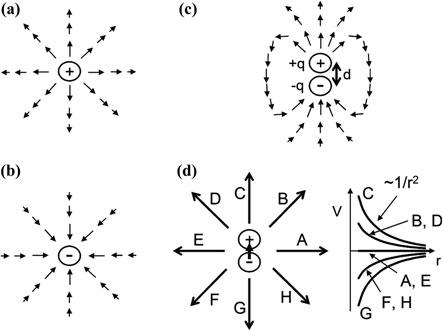
\includegraphics[width=0.7\textwidth]{121.png}
\caption{Se muestran los vectores de campo eléctrico para cargas a) positivas y b) negativas, junto con los de c) un dipolo de dos cargas $+q$ y $-q$, separadas por una distancia $d$, de modo que la magnitud del momento dipolar es $P = qd$. La dirección del momento dipolar se indica mediante la flecha dentro del dipolo en (d). d también muestra el potencial a lo largo de las diferentes direcciones radiales mostradas para este dipolo, y la disminución en $1/r^2$ de cada uno de estos voltajes.}
\label{fig:12.1}
\end{figure}



El potencial de esa carga es
\begin{equation}
V = \frac{kq}{r}, \label{eq:12.2}
\end{equation}

\noindent y, como aquí, el potencial generalmente se define como cero a medida que $r$ tiende a infinito. La diferencia de potencial (o voltaje) entre dos puntos «b» y «a» causada por un campo es
\begin{equation}
\Delta V = V_b - V_a = -\int_{r_a}^{r_b} \vec{\mathbf{E}} \cdot d\vec{\mathbf{r}}, \label{eq:12.3}
\end{equation}

\noindent Esto también se puede expresar como
\begin{equation}
\vec{\mathbf{E}} = -\nabla V, \label{eq:12.4}
\end{equation}

\noindent o en una dimensión como
\begin{equation}
E = -\frac{dV}{dx}. \label{eq:12.5}
\end{equation}

Si hay dos cargas $q$ y $-q$ en el vacío separadas, digamos una distancia $d$ en la dirección del vector unitario $\hat{\mathbf{d}}$ (de modo que el vector entre ellas es $\vec{\mathbf{d}} = d\hat{\mathbf{d}}$), el campo eléctrico es la suma vectorial de las contribuciones de (12.1) y el potencial eléctrico todavía se obtiene utilizando (12.3) (Fig. 12.1c,d). Para $r \gg d$, la expresión para el potencial se puede simplificar para obtener
\begin{equation}
V = k\frac{\vec{\mathbf{P}} \cdot \vec{\mathbf{r}}}{r^3}, \label{eq:12.6}
\end{equation}

\noindent donde $\vec{\mathbf{P}} = q\vec{\mathbf{d}}$ es el vector de momento dipolar eléctrico, que tiene magnitud $P = qd$ y apunta en la dirección de $\vec{\mathbf{d}}$. Si el ángulo entre el vector de dipolo $\vec{\mathbf{P}}$ y el vector de distancia $\vec{\mathbf{r}}$ es $\theta$, entonces esta ecuación se convierte en
\begin{equation}
V = \frac{kP \cos\theta}{r^2}. \label{eq:12.7}
\end{equation}

De manera similar, podemos calcular el momento dipolar para muchas cargas separadas por diversas distancias. La evaluación de los campos causados por tales dipolos eléctricos es de particular valor cuando no hay carga neta en la colección de cargas, como ocurre en casi todas partes del cuerpo.

Consideremos ahora una partícula en movimiento con carga $q$ (en coulombs, $\text{C}$), la corriente, $I = dq/dt$, asociada con tal carga o cargas (que es el cambio de carga por unidad de tiempo), y la densidad de corriente asociada, $J = I/A$ (que es la corriente que fluye por unidad de área $A$). La carga se conserva, lo que significa que no se crea ni se pierde. También significa que la suma vectorial de todas las corrientes que entran en un volumen o en un elemento de volumen pequeño (como un nodo) es cero en estado estacionario (Fig. 12.2). Esta conservación de la corriente (y de la carga) se conoce como la primera ley de Kirchhoff
\begin{equation}
\sum_n I_n = 0. \label{eq:12.8}
\end{equation}

\begin{figure}[htbp]
\centering
  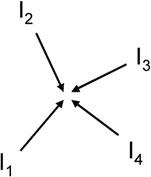
\includegraphics[width=0.55\textwidth]{122.png}
\caption{Primera ley de Kirchhoff, que muestra que la suma algebraica de los flujos de corriente hacia un punto debe ser cero (si la carga no se está acumulando ni agotando en ese punto). (Téngase en cuenta que al menos uno de los flujos de corriente debe ser negativo, es decir, debe apuntar hacia afuera).}
\label{fig:12.2}
\end{figure}



(La dirección del flujo de corriente es importante aquí, a pesar de que la corriente se exprese como un escalar).

Cuando una corriente fluye a lo largo de un material con resistencia $R$ (en ohmios, $\Omega$) (que llamamos $R_{\text{elect}}$ en otros capítulos), hay una caída de voltaje $V$ (en voltios, $\text{V}$) (que llamamos $V_{\text{elect}}$ en otros capítulos) a través del material dada por la ley de Ohm (Fig. 12.3a)
\begin{equation}
V = IR. \label{eq:12.9}
\end{equation}

\begin{figure}[htbp]
\centering
  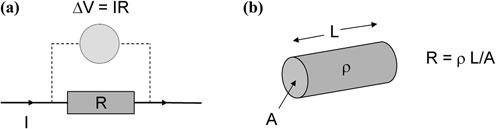
\includegraphics[width=0.8\textwidth]{123.png}
\caption{a) Ley de Ohm y b) evaluación de la resistencia $R$ a partir de la resistividad $\rho$.}
\label{fig:12.3}
\end{figure}



La resistencia es una propiedad extensiva que depende de la propiedad intensiva de resistividad $\rho$ del material, y del área de la sección transversal $A$ y la longitud $L$ de la estructura (Fig. 12.3b)
\begin{equation}
R = \frac{\rho L}{A}. \label{eq:12.10}
\end{equation}

Para un cilindro con radio $a$, tenemos $A = \pi a^2$ y $R = \rho L/\pi a^2$. Más generalmente, para una estructura con sección transversal uniforme, la resistencia $R$ es proporcional a la longitud y podemos definir una resistencia por unidad de longitud
\begin{equation}
r = \frac{R}{L} = \frac{\rho}{A}, \label{eq:12.11}
\end{equation}

\noindent que es igual a $\rho/\pi a^2$ para la conducción a lo largo de un cilindro. La conductancia $G$ (unidades $\text{S}$ (siemens), $1\text{ S} = 1\text{ mho} = 1/\text{ohm} = 1/\Omega$) es $1/R$, la conductividad es $\sigma = 1/\rho$, y la conductancia por unidad de área $g = G/A = 1/RA = 1/\rho L$. En el cuerpo, los iones cargados, como el $\text{Na}^+$, $\text{K}^+$, $\text{Ca}^{2+}$, $\text{Cl}^-$, y las proteínas cargadas negativamente, son los portadores de carga importantes. Los electrones son los portadores de carga en la mayoría de los circuitos electrónicos fabricados por el hombre.

También puede desarrollarse un voltaje o diferencia de potencial $V$ entre dos estructuras, una con una carga $+q$ y la otra con una carga $-q$, debido a los campos eléctricos que van de una a la otra. Este voltaje es
\begin{equation}
V = \frac{q}{C}, \label{eq:12.12}
\end{equation}

\noindent donde $C$ es la capacitancia (en faradios, $\text{F}$) del sistema (llamada $C_{\text{elect}}$ en otros capítulos). La capacitancia $C$ depende de la geometría de estas dos estructuras. Por ejemplo, podrían ser dos placas paralelas o dos cilindros concéntricos (Fig. 12.4), lo cual es similar al axón de una neurona.

Para dos placas paralelas con área $A$ separadas una distancia $b$ por un aislante con constante dieléctrica $\kappa$, vemos
\begin{equation}
C_{\text{parallel plates}} = \frac{\kappa \epsilon_0 A}{b}. \label{eq:12.13}
\end{equation}

\begin{SCfigure}[0.75][htbp]
\centering
  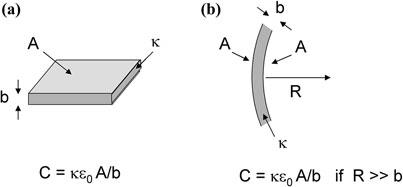
\includegraphics[width=0.6\textwidth]{124.png}
\caption{Capacitancia para a) placas paralelas y b) cortezas cilíndricas.}
\label{fig:12.4}
\end{SCfigure}



\noindent La densidad de carga en cada placa es $\sigma = q/A$.

La suma algebraica de todos los voltajes a lo largo de un circuito de lazo cerrado es igual a cero (Fig. 12.5). Esto se conoce como la segunda ley de Kirchhoff
\begin{equation}
\sum_n V_n = 0. \label{eq:12.14}
\end{equation}

\begin{SCfigure}[0.9][htbp]
\centering
  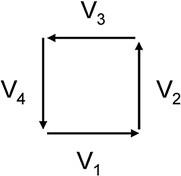
\includegraphics[width=0.5\textwidth]{125.png}
\caption{Segunda ley de Kirchhoff, que muestra que la suma algebraica de las caídas de potencial (voltajes) a lo largo de un lazo cerrado es cero.}
\label{fig:12.5}
\end{SCfigure}



\section{Propiedades eléctricas de los tejidos corporales}

\subsection{Conducción eléctrica a través de la sangre y los tejidos}

Cuando se aplica un voltaje a través de un metal, fluye una corriente porque los electrones se mueven bajo la influencia de un campo eléctrico. Cuando se aplica un voltaje a través de una solución que contiene iones positivos y negativos, fluye corriente porque ambos iones se mueven bajo la influencia del campo eléctrico. La conductividad $\sigma$ de una solución es la suma de las contribuciones al flujo de corriente de cada ion. Para concentraciones bajas de estos iones, esta contribución es proporcional a la concentración $n_i$ de ese ion, con una constante de proporcionalidad $\Lambda_{0,i}$, por lo que
\begin{equation}
\sigma = \sum_i n_i \Lambda_{0,i}. \label{eq:12.15}
\end{equation}

\noindent La Tabla 12.2 proporciona $\Lambda_{0,i}$, la conductancia molar a dilución infinita para varios iones comunes, mientras que la Tabla 12.3 proporciona las concentraciones típicas de iones comunes en la sangre y en las células. La resistencia de una trayectoria se puede determinar usando $\rho = 1/\sigma$ y $R = \rho L/A$ (12.10).

\begin{table}[htbp]
\centering
\caption{Conductancia molar a dilución infinita $\Lambda_{0,i}$ para diferentes iones.}
\label{tab:12.2}
\begin{tabularx}{\textwidth}{X c}
\toprule
Ion & $\Lambda_{0,i}$ ($1/\Omega\cdot\text{m}\cdot\text{M}$) \\
\midrule
$\text{H}^+$ & $34.9$ \\
$\text{OH}^-$ & $19.8$ \\
$\text{Na}^+$ & $5.0$ \\
$\text{Cl}^-$ & $7.6$ \\
\bottomrule
\end{tabularx}
\addvspace{5pt}
\raggedright\small Utilizando datos de [33]
\end{table}

\begin{table}[htbp]
\centering
\caption{Concentraciones iónicas en sangre y citoplasma celular de iones libres.}
\label{tab:12.3}
\begin{tabularx}{\textwidth}{X c c c}
\toprule
Ion & Concentración en sangre & Concentración en citoplasma & Relación \\
\midrule
$\text{Na}^+$ & $145\text{ mM}$ & $12\text{ mM}$ & $12:1$ \\
$\text{K}^+$ & $4\text{ mM}$ & $140\text{ mM}$ & $1:35$ \\
$\text{H}^+$ & $40\text{ nM}$ & $100\text{ nM}$ & $1:2.5$ \\
$\text{Mg}^{2+}$ & $1.5\text{ mM}$ & $0.8\text{ mM}$ & $1.9:1$ \\
$\text{Ca}^{2+}$ & $1.8\text{ mM}$ & $100\text{ nM}$ & $18:1$ \\
$\text{Cl}^-$ & $115\text{ mM}$ & $4\text{ mM}$ & $29:1$ \\
$\text{HCO}_3^-$ & $25\text{ mM}$ & $10\text{ mM}$ & $2.5:1$ \\
\bottomrule
\end{tabularx}
\addvspace{5pt}
\raggedright\small Utilizando datos de [34]
\end{table}

Al igual que muchos materiales, los tejidos corporales tienen propiedades dieléctricas, pero aún poseen cierta conductividad y, por lo tanto, pueden considerarse como dieléctricos con fugas. La resistividad de los tejidos corporales se muestra en la Tabla 12.4 y en la Fig. 12.6.

\begin{figure}[htbp]
\centering
  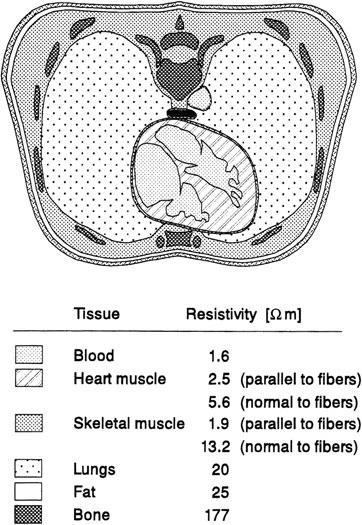
\includegraphics[width=0.45\textwidth]{126.png}
\caption{Sección transversal del tórax, con la resistividad eléctrica de seis tipos de tejidos (De [23]. Utilizado con permiso).}
\label{fig:12.6}
\end{figure}



\begin{table}[htbp]
\centering
\caption{Resistividad a baja frecuencia de algunos tejidos corporales, en $\Omega\cdot\text{m}$.}
\label{tab:12.4}
\begin{tabularx}{\textwidth}{X c}
\toprule
Tejido & Resistividad ($\Omega\cdot\text{m}$) \\
\midrule
Líquido cefalorraquídeo & $0.650$ \\
Plasma sanguíneo & $0.7$ \\
Sangre entera & $1.6$ ($\text{Hct} = 45\%$) \\
Músculo esquelético & \\
\quad -- Longitudinal & $1.25\text{--}3.45$ \\
\quad -- Transversal & $6.75\text{--}18.0$ \\
Hígado & $7$ \\
Pulmón & \\
\quad -- Inspirado & $17.0$ \\
\quad -- Espirado & $8.0$ \\
Tejido neuronal (como en el cerebro) & \\
\quad -- Materia gris & $2.8$ \\
\quad -- Materia blanca & $6.8$ \\
Grasa & $20$ \\
Hueso & $>40$ \\
Piel & \\
\quad -- Húmeda & $10^5$ \\
\quad -- Seca & $10^7$ \\
\bottomrule
\end{tabularx}
\addvspace{5pt}
\raggedright\small Utilizando datos de [3, 9, 23]
\end{table}

\section{Conducción nerviosa}

La Figura 12.7 muestra la estructura de las células nerviosas o neuronas con un núcleo, dendritas que reciben información a través de sinapsis, un axón, y las terminales del axón y sinapsis para la transmisión de señales a otras neuronas. Hay muchos de estos axones neuronales en un nervio. Los axones amielínicos no tienen una vaina que los rodee. Los axones mielínicos tienen vainas de mielina en algunas regiones, las cuales están separadas por los nodos de Ranvier (ron-vii-ei'). Estas vainas están formadas por células de Schwann que están envueltas alrededor del axón (Fig. 12.8), con células envueltas sucesivas separadas en un nodo de Ranvier (Fig. 12.7). Nos concentraremos en cómo viaja un impulso eléctrico a lo largo de tales axones.

\begin{figure}[htbp]
\centering
  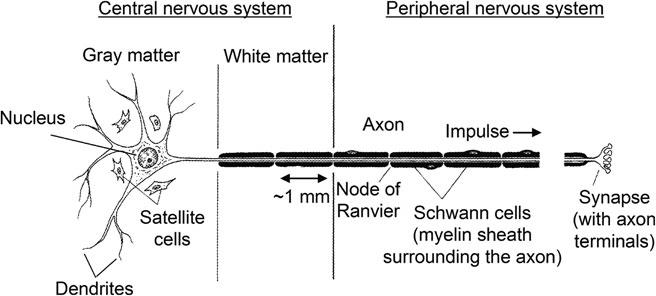
\includegraphics[width=0.8\textwidth]{127.png}
\caption{Estructura de una neurona (De [29]).}
\label{fig:12.7}
\end{figure}

\begin{figure}[htbp]
\centering
  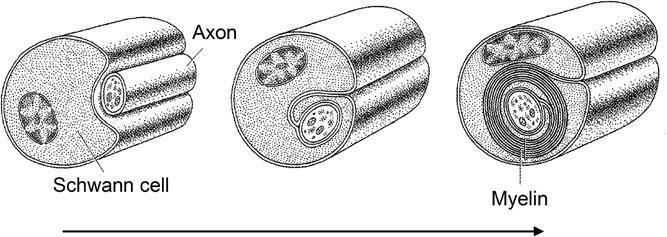
\includegraphics[width=0.8\textwidth]{128.png}
\caption{Envoltura sucesiva de las células de Schwann alrededor del axón de una neurona para formar la vaina de mielina de un nervio mielínico (De [29]).}
\label{fig:12.8}
\end{figure}



Aproximadamente 2/3 de las fibras axónicas en el cuerpo son amielínicas. Tienen radios de $0.05\text{--}0.6\ \mu\text{m}$ y una velocidad de conducción de $u$ (en $\text{m/s}$) $\approx 1.8\sqrt{a}$, donde $a$ es el radio del axón (en $\mu\text{m}$). Las fibras mielínicas tienen radios externos de $0.5\text{--}10\ \mu\text{m}$ y una velocidad de conducción de $u$ (en $\text{m/s}$) $\approx 12(a + b) \approx 17a$, donde $b$ es el espesor de la vaina de mielina (en $\mu\text{m}$) (y $a + b$ es el radio total del axón). El espaciado entre los nodos de Ranvier es $\approx 280a$.

Las neuronas cuyos axones viajan desde las áreas sensoriales hasta la médula espinal se denominan neuronas aferentes o neuronas de entrada o sensoriales. (Son «afectadas» por las condiciones que se perciben). Las neuronas cuyos axones salen de la superficie ventral del tronco del encéfalo y de la médula espinal para transportar señales fuera del sistema nervioso central son neuronas eferentes o neuronas motoras, y estas neuronas ejercen el control motor. (Ellas «efectúan» un cambio). Hay aproximadamente 10 millones de neuronas aferentes, 100 mil millones de neuronas en el cerebro con 100 billones de sinapsis, y medio millón de neuronas eferentes, por lo que hay aproximadamente 20 neuronas sensoriales por cada neurona motora y varios miles de neuronas de procesamiento central por cada neurona de entrada o salida para el procesamiento. Los haces de estos axones neuronales se denominan nervios fuera del cerebro y tractos dentro del cerebro. Los detalles sobre el sistema nervioso se presentan en [25].

Hay aproximadamente $1\text{--}2 \times 10^6$ nervios ópticos a partir de los $1\text{--}2 \times 10^8$ bastones y conos en nuestros ojos, $20\,000$ nervios a partir de las $30\,000$ células ciliadas en nuestros oídos, $2\,000$ nervios a partir de las $10^7$ células olfativas en nuestras narices, $2\,000$ nervios a partir de las $10^8$ células detectoras del gusto en nuestras lenguas, $10\,000$ nervios a partir de las $500\,000$ células sensibles al tacto en todo nuestro cuerpo, y muchos (pero un número incierto de) nervios a partir de las $3 \times 10^6$ células del dolor en todo nuestro cuerpo.

\subsection{Membranas celulares y distribuciones iónicas}

La membrana celular divide las regiones intracelular y extracelular, en las neuronas y otras células. Existen $\text{Na}^+$, $\text{K}^+$, $\text{Cl}^-$, proteínas cargadas negativamente y otras especies cargadas tanto en las neuronas (intracelular) como en el medio extracelular.

Las concentraciones de estos iones son tales que existe neutralidad de carga (es decir, un número igual de cargas positivas y negativas) tanto en el líquido intracelular como en el extracelular. Sin embargo, hay cargas negativas en el interior de la membrana celular y cargas positivas en el exterior de esta membrana que producen un potencial de reposo de $-70\text{ mV}$ (Fig. 12.9). Esto significa que el medio intracelular está a $-70\text{ mV}$, cuando el potencial extracelular se define arbitrariamente como $0\text{ V}$, como es costumbre. Solo las diferencias de potencial son significativas, por lo que no limitamos el análisis al fijar el potencial extracelular. Este potencial de reposo es la diferencia de potencial habitual cuando no hay una actividad neuronal inusual. Esto se conoce como el estado polarizado. (La propagación de una señal eléctrica constituiría una actividad inusual).

\begin{SCfigure}[0.8][htbp]
\centering
  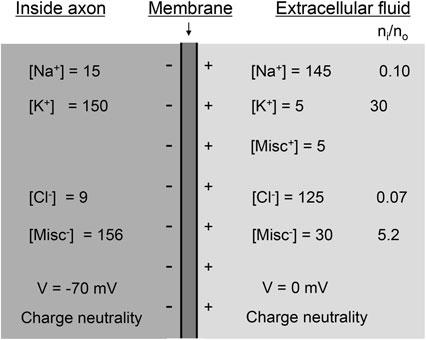
\includegraphics[width=0.55\textwidth]{129.png}
\caption{Concentraciones iónicas (en $\text{mmol/L}$) en una célula nerviosa de axón de mamífero típica ($n_i$) y en el líquido extracelular que la rodea ($n_o$), y sus relaciones ($n_i/n_o$) (Basado en [17, 18]).}
\label{fig:12.9}
\end{SCfigure}



Si bien existe neutralidad de carga tanto dentro como fuera de la membrana, las concentraciones de cada ion no son iguales dentro y fuera de la célula, como veremos. Las diferencias en las concentraciones iónicas dentro y fuera de la membrana celular se deben a un equilibrio dinámico. Cuando hay cambios en la permeabilidad de la membrana celular a diferentes especies cargadas, se producen desequilibrios transitorios de carga neta que modifican el potencial a través de la membrana celular. Un aumento en el potencial de membrana desde $-70\text{ mV}$, como el que llega a $-60\text{ mV}$ en la Fig. 12.10, se conoce como despolarización, mientras que una disminución desde $-70\text{ mV}$ a, por ejemplo, $-80\text{ mV}$ se denomina hiperpolarización. La despolarización se debe al flujo neto de cargas positivas hacia la célula o de cargas negativas a regiones fuera de ella. La hiperpolarización se debe al flujo neto de cargas negativas hacia el interior de la célula o de cargas positivas hacia el exterior. Tales cambios en la permeabilidad iónica se denominan a menudo cambios en el canal iónico.

\begin{figure}[htbp]
\centering
  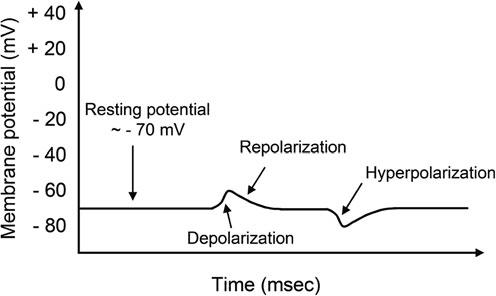
\includegraphics[width=0.8\textwidth]{1210.png}
\caption{El potencial de reposo de la membrana de $-70\text{ mV}$ (dentro de la membrana en relación con el exterior, siempre fijo a $0\text{ mV}$) ---el estado polarizado--- junto con las perturbaciones del potencial que muestran la despolarización (aumentos de voltaje desde el valor del potencial de reposo), la repolarización (retorno al potencial de reposo) y la hiperpolarización (disminuciones desde el potencial de reposo).}
\label{fig:12.10}
\end{figure}



La Figura 12.9 también muestra las concentraciones de algunas de las especies cargadas importantes dentro y fuera de la célula en condiciones de reposo (es decir, polarizadas). Vemos que hay mucho más $\text{Na}^+$ afuera ($145\text{ mmol/L}$) que adentro ($15\text{ mmol/L}$) de la célula, pero mucho más $\text{K}^+$ adentro ($150\text{ mmol/L}$) que afuera ($5\text{ mmol/L}$). Incluyendo diversos iones positivos fuera de la célula, hay $165\text{ mmol/L}$ de iones positivos tanto dentro como fuera de la célula. De manera similar, hay mucho más $\text{Cl}^-$ afuera ($125\text{ mmol/L}$) que adentro ($9\text{ mmol/L}$) de la célula, pero muchos más iones negativos diversos (incluyendo proteínas) adentro ($156\text{ mmol/L}$) que afuera ($30\text{ mmol/L}$). También hay $165\text{ mmol/L}$ de iones negativos tanto dentro como fuera de la célula.

Existen varias fuerzas impulsoras que determinan las concentraciones iónicas, en general, y estas concentraciones intracelulares y extracelulares, en particular:

1. Existe la tendencia natural a que las concentraciones sean uniformes en todas partes, por lo que cuando hay gradientes de concentración a través de la membrana celular se producen flujos de estas especies desde las regiones de mayor concentración hacia las regiones de menor concentración, para igualar las concentraciones intracelular y extracelular. Esto se describe mediante la primera ley de difusión de Fick (7.64), $J_{\text{diff}} = -D_{\text{diff}} dn/dx$, donde $J_{\text{diff}}$ es el flujo de iones en la dirección $x$ (el número de iones que fluyen a través de un área unitaria en un tiempo unitario), $D_{\text{diff}}$ es la constante de difusión, $n$ es la concentración local de iones y $dn/dx$ es el gradiente de concentración local.

2. Debido a que el potencial es negativo dentro de la célula, esperaríamos que los iones positivos entren en la célula y sean más dominantes en el líquido intracelular que en el extracelular y que existan tales gradientes de concentración; esto es cierto para el $\text{K}^+$ pero no para el $\text{Na}^+$. De manera similar, esperamos que los iones negativos salgan de la célula debido al potencial de reposo y sean más dominantes fuera de la célula que dentro de ella ---y nuevamente que existan gradientes de concentración; esto es cierto para el $\text{Cl}^-$ pero no para las proteínas cargadas negativamente, que constituyen la mayor parte de los iones negativos diversos.

Cuando las especies cargadas están en un campo eléctrico, se aceleran y eventualmente alcanzan una velocidad de deriva en estado estacionario, $\vec{\mathbf{v}}_{\text{drift}}$, debido a las colisiones que actúan como una fuerza de arrastre. Como se muestra en el problema 12.7, la velocidad de deriva de un ion dado es
\begin{equation}
\vec{\mathbf{v}}_{\text{drift}} = \mu \vec{\mathbf{E}}. \label{eq:12.16}
\end{equation}

% ---- Bloque 2: temp_cap_12_pag_830_840.tex ----
donde $\mu$ se denomina la movilidad y $E$ es el campo eléctrico. El flujo de iones debido a este campo eléctrico es
\begin{equation}
J_{\text{elect}} = n v_{\text{drift}} = n \mu E. \label{eq:12.17}
\end{equation}

3. La permeabilidad de la membrana celular y los procesos activos hacen que las concentraciones de iones en ambos lados de la membrana se desvíen de los valores esperados a partir de la difusión y el movimiento de cargas en campos eléctricos. Las membranas celulares son permeables al $\text{K}^+$ y al $\text{Cl}^-$, lo que explica por qué se comportan como se espera. Las proteínas nunca son permeables a la membrana celular, razón por la cual la concentración de iones de proteínas negativas es inesperadamente alta en el interior. El mecanismo químico denominado bomba de $\text{Na}^+$ (o bomba de $\text{Na}^+$--$\text{K}^+$) transporta activamente $3\text{Na}^+$ desde el interior hacia el exterior de la célula por cada $2\text{K}^+$ que transporta desde el exterior hacia el interior de la célula; esto mantiene al $\text{Na}^+$ fuera de la célula y al $\text{K}^+$ dentro.

La alta concentración de $\text{Na}^+$ fuera de la célula es el resultado de la bomba de $\text{Na}^+$ que lucha contra las fuerzas eléctricas impulsoras y la tendencia a igualar las concentraciones (Fig. 12.11). La alta concentración de $\text{K}^+$ dentro de la célula es el resultado de las fuerzas eléctricas y de la bomba de $\text{Na}^+$ que luchan contra la tendencia a igualar las concentraciones. La alta concentración de $\text{Cl}^-$ fuera de la célula es el resultado de las fuerzas eléctricas que luchan contra la tendencia a igualar las concentraciones. La concentración de iones de proteínas negativas es inesperadamente alta en el interior porque son grandes y no son permeables a la membrana celular.

La Figura 12.12 representa las direcciones de movimiento de moléculas cargadas y neutras tanto para el movimiento térmico aleatorio en la difusión como para el efecto dirigido debido a un campo eléctrico. La Figura 12.13 muestra cómo cambia una banda concentrada de moléculas cargadas y neutras debido a la difusión o a un campo eléctrico.

\begin{figure}[htbp]
\centering
  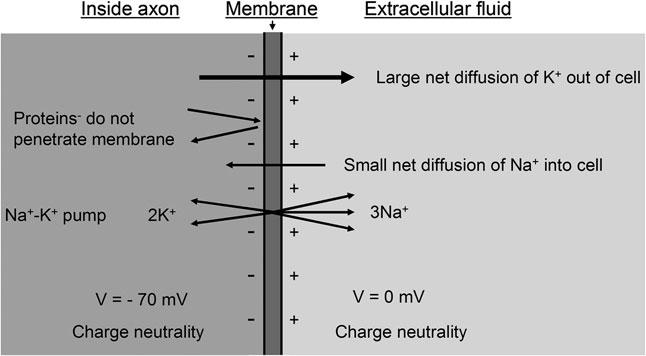
\includegraphics[width=0.8\textwidth]{1211.png}
\caption{Mecanismos para el flujo de iones a través de una membrana celular polarizada que determinan el potencial de membrana en reposo.}
\label{fig:12.11}
\end{figure}

\begin{figure}[htbp]
\centering
  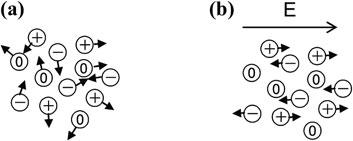
\includegraphics[width=0.8\textwidth]{1212.png}
\caption{La dirección del movimiento de moléculas cargadas y neutras debido a a) difusión únicamente (en un instante dado) y b) un campo eléctrico únicamente.}
\label{fig:12.12}
\end{figure}

\begin{figure}[htbp]
\centering
  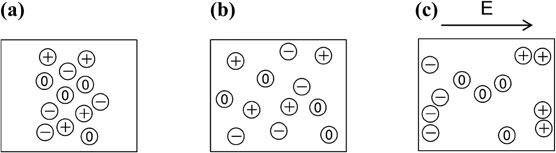
\includegraphics[width=0.8\textwidth]{1213.png}
\caption{Una banda inicial de moléculas cargadas y neutras (en a) cambia de manera muy diferente por la dispersión térmica uniforme en la difusión (en b) y la separación causada por un campo eléctrico (en c). a) Antes, b) Después, solo difusión, c) Después, solo campo eléctrico.}
\label{fig:12.13}
\end{figure}



\subsection{Distribuciones iónicas (Tema avanzado)}
\label{subsec:ionic_distributions}

¿Cuáles son las distribuciones iónicas esperadas debido al potencial de membrana? Primero, consideremos las distribuciones esperadas para varias condiciones de estado estacionario para un ion dado. En estado estacionario, el flujo neto de iones hacia cualquier región es cero, por lo que $J_{\text{diff}} + J_{\text{elect}} = 0$ y, utilizando (7.64) y (12.17), vemos que
\begin{equation}
D_{\text{diff}} \frac{dn}{dx} = n \mu E. \label{eq:12.18}
\end{equation}

(En estado estacionario, $n$ no depende del tiempo, por lo que la derivada parcial en (7.64) no es necesaria aquí).

El coeficiente de difusión, $D_{\text{diff}}$, y la movilidad, $\mu$, están en realidad estrechamente relacionados. Considere un cilindro de área de sección transversal $A$ y longitud $dx$ a lo largo de la dirección $x$ que contiene una densidad $n$ de iones de carga $q$. Cuando se aplica un campo eléctrico $E$ a lo largo de la dirección $x$, los iones en el cilindro experimentan una fuerza $(nq)(A\,dx)E$, donde $nq$ es la carga total por unidad de volumen y $A\,dx$ es el volumen. La fuerza mecánica sobre este cilindro se debe a la diferencia entre la presión $\times$ área en una pared lateral, $A P(x)$, y la de la otra pared lateral, $A P(x + dx) = A[P(x) + (dP/dx)dx]$, o $-A(dP/dx)dx$. La suma de estas fuerzas es cero en estado estacionario, por lo que $dP/dx = nqE$. Utilizando la ley de los gases ideales (7.2) $P = n k_B T$ (que aquí es una aproximación y donde $n$ es ahora el número de moléculas por unidad de volumen porque se usa $k_B$ en lugar de la constante de los gases $R$), vemos que $dP/dx = k_B T (dn/dx)$ o $k_B T (dn/dx) = nqE$. Comparando esto con (12.18), se obtiene la ecuación de Einstein
\begin{equation}
\mu = \frac{q D_{\text{diff}}}{k_B T}, \label{eq:12.19}
\end{equation}
un resultado que utilizaremos pronto.

Ahora consideremos la corriente de carga debida a dos iones, uno de carga $q$ (que diremos que es $>0$), con densidad $n_+$ y movilidad $\mu_+$, y el otro de carga $-q$, con densidad $n_-$ y movilidad $\mu_-$. (Ahora definiremos las movilidades como positivas, de modo que para este ion negativo $v_{\text{drift}} = -\mu_- E$). Si estos son los únicos dos iones, la neutralidad de carga da $n_+ = n_- = n$. El flujo de partículas de cada uno está determinado por el gradiente de concentración de cada uno y el movimiento de cada uno en un campo eléctrico. El flujo de carga $j_{\text{flux}}$ (o densidad de corriente) es la carga del ion $\times$ el flujo del ion. Para el ion positivo: $j_{\text{flux},+} = q(J_{\text{diff},+} + J_{\text{elect},+}) = -q D_{\text{diff},+}(dn/dx) + qn\mu_+ E$ y para el ion negativo es: $j_{\text{flux},-} = -q(J_{\text{diff},-} + J_{\text{elect},-}) = q D_{\text{diff},-}(dn/dx) + qn\mu_- E$, por lo que la densidad de corriente total es
\begin{equation}
j_{\text{flux}} = -q(D_{\text{diff},+} - D_{\text{diff},-})\frac{dn}{dx} + qn(\mu_+ + \mu_-)E, \label{eq:12.20}
\end{equation}
la cual se conoce como la ecuación de Nernst--Planck. Esta también se puede escribir como
\begin{equation}
j_{\text{flux}} = qn(\mu_+ + \mu_-) \left[ E - \frac{D_{\text{diff},+} - D_{\text{diff},-}}{\mu_+ + \mu_-} \frac{d \ln n}{dx} \right], \label{eq:12.21}
\end{equation}
donde hemos expresado $(dn/dx)/n$ como $d \ln n/dx$. El prefactor en el lado derecho es la conductividad, $\sigma = qn(\mu_+ + \mu_-)$. (Además, el factor $\Lambda_{0,i}$ en (12.15) claramente es igual a $q_i \mu_i$).

Cuando no hay flujo de corriente neto, vemos
\begin{equation}
E = \frac{D_{\text{diff},+} - D_{\text{diff},-}}{\mu_+ + \mu_-} \frac{d \ln n}{dx}. \label{eq:12.22}
\end{equation}

Por lo tanto, el voltaje entre dos puntos, como desde el interior (con el subíndice $i$) de la membrana hacia el exterior (con el subíndice $o$), es
\begin{align}
V = V_i - V_o &= - \int_{\text{exterior}}^{\text{interior}} E \, dx \label{eq:12.23} \\
&= - \frac{D_{\text{diff},+} - D_{\text{diff},-}}{\mu_+ + \mu_-} \int_{\text{exterior}}^{\text{interior}} \frac{d \ln n}{dx} \, dx \label{eq:12.24} \\
&= - \frac{D_{\text{diff},+} - D_{\text{diff},-}}{\mu_+ + \mu_-} \ln(n_i / n_o). \label{eq:12.25}
\end{align}

Utilizando la relación de Einstein, (12.19), sabemos que $D_{\text{diff}} = \mu k_B T / q$, y por lo tanto
\begin{equation}
V = -\frac{k_B T}{q} \frac{\mu_+ - \mu_-}{\mu_+ + \mu_-} \ln(n_i / n_o). \label{eq:12.26}
\end{equation}
Esta es la ecuación de Nernst.

Apliquemos esto a una membrana que es impermeable a los iones negativos, de modo que $\mu_- = 0$ y
\begin{equation}
V = -\frac{k_B T}{q} \ln(n_i / n_o). \label{eq:12.27}
\end{equation}

Llamando a la carga $q = Ze$, donde $e$ es la magnitud de una carga elemental (electrón o protón), vemos que
\begin{equation}
\frac{n_i}{n_o} = \exp\left( -Ze(V_i - V_o)/k_B T \right). \label{eq:12.28}
\end{equation}
Esta relación se conoce como la relación de Donnan y este se conoce como el equilibrio de Donnan.

Las densidades iónicas se consideran constantes tanto en la región interior como en la exterior.

Esta relación también se obtiene mediante la distribución de Maxwell--Boltzmann, que da la probabilidad $P(E, T)$ de que un estado con energía $E$ esté ocupado en equilibrio térmico a temperatura $T$.
\begin{equation}
P(E, T) = A \exp(-E/k_B T). \label{eq:12.29}
\end{equation}

La energía potencial de la carga es $E = ZeV$. Si una especie dada estuviera en equilibrio térmico, esperaríamos que su concentración $n$ fuera proporcional a $\mathrm{e}^{-ZeV_{\mathrm{local}}/k_B T}$, donde $V_{\mathrm{local}}$ es el potencial local, o más exactamente
\begin{equation}
n = n_{\infty} \exp(-ZeV_{\text{local}}/k_B T), \label{eq:12.30}
\end{equation}
donde $n_{\infty}$ es la concentración muy lejos, donde el potencial es cero. En particular, esperaríamos que la relación de las concentraciones de cada ion dentro y fuera de la célula dé (12.28).

Esta relación de Donnan incluye la física de las dos primeras fuerzas impulsoras explicadas anteriormente, así como la física del equilibrio térmico. Para el potencial en reposo $V_i - V_o = -70\text{ mV}$ a $T = 310\text{ K}$ (temperatura corporal central) y $Z = +1$, esperamos $n_i/n_o = 13.7$ para este equilibrio de «Donnan»; para el $\text{Na}^+$ esta relación es $15/145 = 0.103$ y para el $\text{K}^+$ es $150/5 = 30$. Para $Z = -1$ esperamos $n_i/n_o = 1/13.7 = 0.073$; para el $\text{Cl}^-$ esta relación es $9/125 = 0.072$ y para los iones de carga negativa simple misceláneos es $156/30 = 5.2$. Existe un acuerdo relativamente bueno para el $\text{K}^+$ y el $\text{Cl}^-$, y un gran desacuerdo para el $\text{Na}^+$ y los misceláneos$^-$ por las razones expuestas anteriormente, como la bomba de $\text{Na}^+$ para el $\text{Na}^+$. (El acuerdo no es perfecto para el $\text{K}^+$ porque la bomba de $\text{Na}^+$ introduce $\text{K}^+$ en la célula).

El potencial teórico de Nernst $V_{\text{Nernst}}$ es el potencial que conduciría a las relaciones de concentración observadas
\begin{equation}
\left( \frac{n_i}{n_o} \right)_{\text{observado}} = \exp\left( -Ze V_{\text{Nernst}}/k_B T \right). \label{eq:12.31}
\end{equation}
Para el $\text{Na}^+$ es de $61\text{ mV}$, para el $\text{K}^+$ es de $-91\text{ mV}$ y para el $\text{Cl}^-$ es de $-70\text{ mV}$.

Cuando la ecuación de Nernst (12.27) se generaliza para incluir los efectos de múltiples iones, como $\text{Na}^+$, $\text{K}^+$ y $\text{Cl}^-$, y la permeabilidad de la membrana, se obtiene la ecuación de voltaje de Goldman
\begin{equation}
V = -\frac{k_B T}{q} \ln\left( \frac{p_{\text{Na}} n_{\text{Na},i} + p_{\text{K}} n_{\text{K},i} + p_{\text{Cl}} n_{\text{Cl},i}}{p_{\text{Na}} n_{\text{Na},o} + p_{\text{K}} n_{\text{K},o} + p_{\text{Cl}} n_{\text{Cl},o}} \right), \label{eq:12.32}
\end{equation}

con las permeabilidades de la membrana $p$ (y con los subíndices $i$ para el interior y $o$ para el exterior). Para las neuronas y las células sensoriales, la permeabilidad para el $\text{Cl}^-$ es tan pequeña que a menudo se puede despreciar, y encontramos:
\begin{equation}
V = -\frac{k_B T}{q} \ln\left( \frac{p_{\text{Na}} n_{\text{Na},i} + p_{\text{K}} n_{\text{K},i}}{p_{\text{Na}} n_{\text{Na},o} + p_{\text{K}} n_{\text{K},o}} \right) \label{eq:12.33}
\end{equation}
o
\begin{equation}
V = -\frac{k_B T}{q} \ln\left( \frac{\alpha n_{\text{Na},i} + n_{\text{K},i}}{\alpha n_{\text{Na},o} + n_{\text{K},o}} \right), \label{eq:12.34}
\end{equation}
con $\alpha = p_{\text{Na}}/p_{\text{K}}$. Utilizando las concentraciones anteriores y $\alpha = 0.02$, esta diferencia de potencial en reposo es de $-75\text{ mV}$, lo que está más cerca del potencial en reposo real que el $V_{\text{Nernst}} = -91\text{ mV}$ para el $\text{K}^+$.

\subsection{Ecuación de Poisson--Boltzmann (Tema avanzado)}
\label{subsec:poisson_boltzmann}

Hasta ahora hemos determinado las relaciones de concentración para un potencial dado. Un problema más general, y que está un poco más allá de nuestro alcance, consiste en determinar el potencial $V$ utilizando (12.1) y (12.3) y las densidades de las cargas en la región. En otras palabras, también necesitamos acoplar el potencial con las distribuciones de los iones.

Al integrar el campo sobre una superficie $a$, como una esfera, alrededor de la carga $q$, la ley de Coulomb (12.1) se convierte en la ley de Gauss
\begin{equation}
\oint \vec{\mathbf{E}} \cdot d\vec{\mathbf{a}} = \frac{1}{\epsilon_0 \epsilon} q. \label{eq:12.35}
\end{equation}

Esto se puede convertir a la forma diferencial
\begin{equation}
\nabla \cdot \vec{\mathbf{E}} = \frac{1}{\epsilon_0 \epsilon} \rho, \label{eq:12.36}
\end{equation}

donde $\rho$ es la densidad de carga
\begin{equation}
\rho = \sum_i Z_i e n_i. \label{eq:12.37}
\end{equation}

En una dimensión, esta forma de la ley de Gauss se convierte en
\begin{equation}
\frac{dE}{dx} = \frac{1}{\epsilon_0 \epsilon} \rho. \label{eq:12.38}
\end{equation}

Utilizando la relación entre el campo eléctrico y el potencial (12.4) y (12.5), estas se convierten en la ecuación de Poisson
\begin{equation}
\nabla^2 V = -\frac{1}{\epsilon_0 \epsilon} \rho, \label{eq:12.39}
\end{equation}

la cual en una dimensión se convierte en:
\begin{equation}
\frac{d^2V}{dx^2} = -\frac{1}{\epsilon_0 \epsilon} \rho. \label{eq:12.40}
\end{equation}

Al combinar esto con la relación de Maxwell--Boltzmann (12.30) y con (12.37), se obtiene la ecuación de Poisson--Boltzmann:
\begin{equation}
\nabla^2 V = -\frac{1}{\epsilon_0 \epsilon} \sum_i Z_i e n_{i,0} \exp(-Z_i e V / k_B T). \label{eq:12.41}
\end{equation}

Sin estas cargas libres y móviles en solución, el potencial de una carga $Ze$, como un ion en solución, viene dado por (12.2), $V = Ze / (4\pi\epsilon_0\epsilon r)$. Estas cargas móviles apantallan o protegen parcialmente el potencial debido a esta carga, como se observa al resolver la ecuación de Poisson--Boltzmann. Cuando $Z_i e V / k_B T \ll 1$, podemos utilizar $\exp(x) \approx 1 + x$ para $|x| \ll 1$ para aproximar la exponencial en (12.41) como $1 - Z_i e V / k_B T$. Esto da
\begin{equation}
\nabla^2 V = -\frac{1}{\epsilon_0 \epsilon} \sum_i Z_i e n_{i,0} + \frac{1}{\epsilon_0 \epsilon} \sum_i \frac{Z_i^2 e^2 n_{i,0} V}{k_B T}. \label{eq:12.42}
\end{equation}

En regiones de carga neutra, el primer término en el lado derecho se anula, dejando
\begin{equation}
\nabla^2 V = \frac{e^2}{\epsilon_0\epsilon k_B T} \left[ \sum_i Z_i^2 n_{i,0} \right] V \label{eq:12.43}
\end{equation}

o
\begin{equation}
\nabla^2 V = \kappa^2 V, \label{eq:12.44}
\end{equation}

donde $\kappa$ es el parámetro de Debye--Hückel dado por
\begin{equation}
\kappa^2 = \frac{e^2}{\epsilon_0\epsilon k_B T} \sum_i Z_i^2 n_{i,0} \label{eq:12.45}
\end{equation}

Esto se resuelve en tres dimensiones (ver el Problema 12.8 y el Apéndice C) para obtener el potencial
\begin{equation}
V(r) = \frac{Ze}{4\pi\epsilon_0\epsilon r} \exp(-\kappa r). \label{eq:12.46}
\end{equation}
Esto significa que la carga se apantalla más allá de la longitud de Debye--Hückel dada por el radio $1/\kappa$.

\subsection{Tipos de excitaciones de la membrana celular}
\label{subsec:types_of_cell_membrane_excitations}

Existen dos tipos cualitativamente diferentes de excitaciones del axón: potenciales graduados y potenciales de acción.

Los potenciales graduados (Fig. 12.14) son perturbaciones menores en el potencial de membrana debidas a la unión de neurotransmisores, la estimulación de la recepción sensorial o la fuga espontánea de iones a través de la membrana celular. No se necesita ningún umbral para estimular un potencial graduado. Duran desde $5\text{ ms}$ hasta varios minutos. Los potenciales graduados pueden ser tanto despolarizaciones como hiperpolarizaciones de la membrana. Los potenciales graduados sucesivos pueden sumarse entre sí. Se propagan solo distancias cortas a lo largo de la membrana antes de decaer.

\begin{figure}[htbp]
\centering
  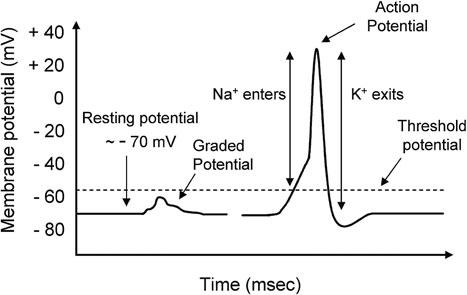
\includegraphics[width=0.7\textwidth]{1214.png}
\caption{Los potenciales graduados (subumbrales) y los potenciales de acción (por encima del umbral).}
\label{fig:12.14}
\end{figure}



Los potenciales de acción son cualitativamente diferentes de los potenciales graduados en todos los aspectos (Fig. 12.14). Inicialmente presentan despolarizaciones relativamente grandes de aproximadamente $15$--$20\text{ mV}$ por encima del valor en reposo de $-70\text{ mV}$ hasta un umbral de aproximadamente $-55\text{ mV}$. A este potencial umbral, la membrana celular se abre permitiendo el transporte de $\text{Na}^+$. El potencial dura de $1$ a $5\text{ ms}$ y siempre implica la despolarización de la membrana. Cada potencial de acción abre la membrana celular y no se suman entre sí. No hay disminución en el potencial a lo largo de toda la longitud del axón de la célula neuronal, ya que este potencial de acción conduce a la propagación de una señal eléctrica a lo largo del axón. Analizaremos esto cuantitativamente en la Secc. 12.3.3.

La Figura 12.14 muestra la secuencia temporal del potencial de acción en un punto del axón. Después de alcanzar el umbral de aproximadamente $-55\text{ mV}$, los canales de $\text{Na}^+$ dependientes de voltaje comienzan a abrirse y el $\text{Na}^+$ entra rápidamente en la célula debido al potencial negativo. Hay un exceso de iones positivos dentro de la célula y el potencial se vuelve positivo, aumentando hasta aproximadamente $20\text{ mV}$. Esto hace que los iones positivos, como el $\text{K}^+$, salgan de la célula y el potencial disminuya por debajo del potencial umbral hasta el potencial en reposo (lo cual es un sobreimpulso). Este pulso eléctrico viaja a lo largo del axón. La Figura 12.15 muestra la despolarización y repolarización y el flujo de iones para el músculo cardíaco. El movimiento local de los iones cerca de la membrana se muestra en la Fig. 12.16 durante la propagación de la señal.

\begin{SCfigure}[1.3][htbp]
\centering
  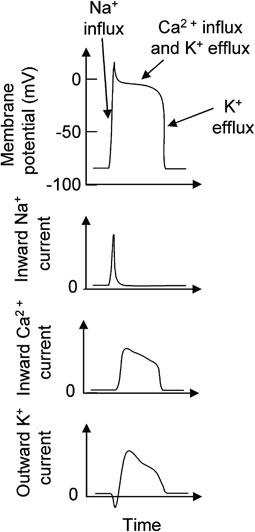
\includegraphics[width=0.35\textwidth]{1215.png}
\caption{La despolarización y repolarización del músculo cardíaco, junto con los flujos de iones $\text{Na}^+$, $\text{Ca}^{2+}$ y $\text{K}^+$. El flujo hacia el interior de $\text{Na}^+$ y $\text{Ca}^{2+}$ aumenta el potencial y el flujo hacia el exterior de $\text{K}^+$ lo disminuye (Basado en [22]).}
\label{fig:12.15}
\end{SCfigure}

\begin{figure}[htbp]
\centering
  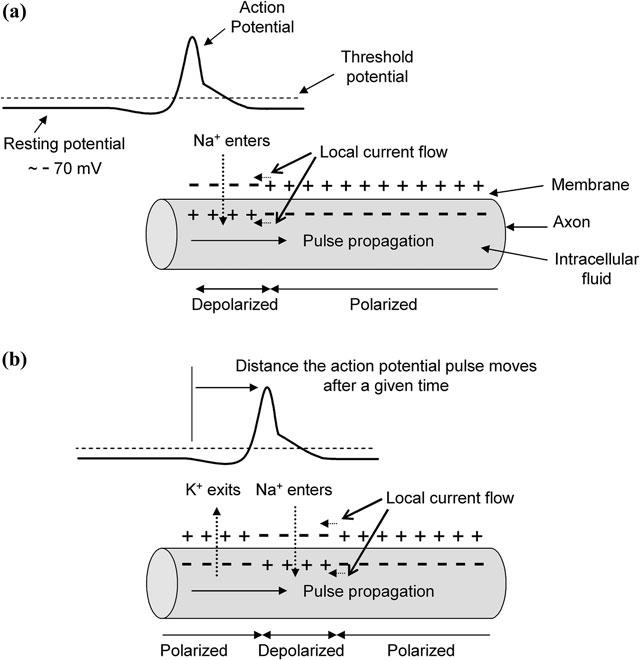
\includegraphics[width=0.55\textwidth]{1216.png}
\caption{El flujo de iones a través de la membrana durante la propagación del potencial de acción a) en un tiempo dado y b) en un tiempo posterior.}
\label{fig:12.16}
\end{figure}



\subsection{Modelo de conducción eléctrica a lo largo de un axón}
\label{subsec:model_of_electrical_conduction}

Los axones neuronales se pueden tratar como un cable eléctrico con parámetros pasivos que lo caracterizan por unidad de longitud, con una excepción notable. La resistencia de los fluidos dentro del axón, $r_i$, fuera del axón, $r_o$, y de la membrana del axón, $r_m$, se puede caracterizar por unidad de longitud del axón. El axón también se puede caracterizar por su capacitancia por unidad de longitud, $c_m$. El axón se puede modelar entonces mediante el cable eléctrico de la Fig. 12.17 con unidades repetitivas. Hasta ahora, esta descripción solo puede explicar las características de decaimiento de los potenciales graduados. Como veremos, la propagación de los potenciales de acción a lo largo del axón requiere el flujo de corriente adicional de iones a través de la membrana del axón (ver [5, 17--19, 23]).

\begin{figure}[htbp]
\centering
  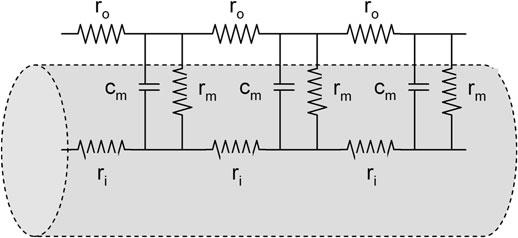
\includegraphics[width=0.8\textwidth]{1217.png}
\caption{Modelo de circuito distribuido de un axón, con la resistencia dentro del axón $r_i$, la resistencia de la membrana $r_m$ y la capacitancia $c_m$, y la resistencia fuera del axón $r_o$, cada una por unidad de longitud.}
\label{fig:12.17}
\end{figure}



\subsection{Propiedades de las neuronas y los nervios}
\label{subsec:properties_of_neurons_and_nerves}

Los parámetros de la Tabla 12.5 para axones nerviosos no mielinizados y mielinizados nos ayudarán a comprender las propiedades eléctricas del axón como lo haríamos con cualquier cable con una resistencia y capacitancia distribuidas. A partir de la Tabla 12.5, la resistividad para un nervio no mielinizado es típicamente $\rho_i = 0.5\ \Omega\cdot\text{m}$ y el radio del axón es $a = 5 \times 10^{-6}\text{ m}$, por lo que la resistividad dentro del axón por unidad de longitud a lo largo del axón es
\begin{equation}
r_i = \frac{\rho_i}{\pi a^2} = \frac{0.5\ \Omega\cdot\text{m}}{\pi (5 \times 10^{-6}\text{ m})^2} = 6.4 \times 10^9\ \Omega/\text{m} = 6.4 \times 10^3\ \Omega/\mu\text{m}. \label{eq:12.47}
\end{equation}

\begin{table}[htbp]
\centering
\caption{Parámetros típicos para nervios no mielinizados y mielinizados.}
\label{tab:12.5}
\begin{tabularx}{\textwidth}{X c c}
\toprule
 & No mielinizado & Mielinizado \\
\midrule
Radio interno del axón ($\text{m}$) & & \\
\quad $a$ & $5 \times 10^{-6}$ & $5 \times 10^{-6}$ \\
Espesor de la membrana/mielina ($\text{m}$) & & \\
\quad $b$ & $6 \times 10^{-9}$ & $2 \times 10^{-6}$ \\
Resistividad del axoplasma ($\Omega\cdot\text{m}$) & & \\
\quad $\rho_i$ & $1.1$ & $1.1$ \\
Constante dieléctrica de la membrana ($\text{s/}\Omega\cdot\text{m}$) & & \\
\quad $\kappa\epsilon_0$ & $6.20 \times 10^{-11}$ & $6.20 \times 10^{-11}$ \\
Resistividad de la membrana/mielina ($\Omega\cdot\text{m}$) & & \\
\quad $\rho_m$ & $10^7$ & $10^7$ \\
Resistencia por unidad de longitud del fluido ($\Omega/\text{m}$)$^a$ & & \\
\quad $r$ & $6.37 \times 10^9$ & $6.37 \times 10^9$ \\
Conductividad/longitud de la membrana del axón ($\text{mho/m}$) & & \\
\quad $g_m$ & $1.25 \times 10^{-4}$ & $3 \times 10^{-7}$ \\
Capacitancia/longitud del axón ($\text{F/m}$) & & \\
\quad $c_m$ & $3 \times 10^{-7}$ & $8 \times 10^{-10}$ \\
\bottomrule
\end{tabularx}
\addvspace{5pt}
{\raggedright\small De [6, 7, 17] \\
$^a$Fluido tanto dentro como fuera del axón. \par}
\end{table}

La resistividad de la membrana es $\rho_m = 1.6 \times 10^7\ \Omega\cdot\text{m}$, el espesor de la membrana es $b = 6 \times 10^{-9}\text{ m}$, y el área de la sección transversal de la membrana normal al eje del axón es $A = 2\pi a b$. Por lo tanto, la resistividad de la membrana por unidad de longitud a lo largo del axón es
\begin{align}
r_m = \frac{\rho_m}{2\pi a b} &= \frac{1.6 \times 10^7\ \Omega\cdot\text{m}}{2\pi(5 \times 10^{-6}\text{ m})(6 \times 10^{-9}\text{ m})} \label{eq:12.48} \\
&= 8 \times 10^{19}\ \Omega/\text{m} = 8 \times 10^{13}\ \Omega/\mu\text{m}. \label{eq:12.49}
\end{align}
Esta resistividad es tan alta que para una caída de voltaje dada a lo largo del axón, el flujo de corriente a lo largo de la membrana es despreciable en comparación con el del fluido.

La resistencia transversal a través de la membrana es $(\rho_m b)/A_{\text{transversal}}$, por lo que la conductancia por unidad de área es
\begin{equation}
g_m = \frac{1}{\rho_m b}, \label{eq:12.50}
\end{equation}
donde la conductancia es el recíproco de la resistencia.

Debido a que el radio del axón $a$ de un axón no mielinizado es mucho mayor que el espesor de la membrana $b$, la membrana cilíndrica se puede desenrollar a lo largo de su longitud (muy similar a la Fig. 12.4) y modelarse con gran éxito como un capacitor de placas paralelas, con separación de placas $b$ y área $A = 2\pi a L$, donde $L$ es la longitud de la unidad de axón. El material en la membrana del axón tiene una constante dieléctrica $\kappa = 7$, por lo que con $\epsilon_0 = 8.85 \times 10^{-12}\text{ s/}\Omega\cdot\text{m}$ vemos que $\kappa\epsilon_0 = 6.20 \times 10^{-11}\text{ s/}\Omega\cdot\text{m}$. A partir de (12.13), la capacitancia por unidad de longitud de un axón no mielinizado es
\begin{align}
C_{\text{placas paralelas, por longitud}} = \frac{C_{\text{placas paralelas}}}{L} &= \frac{2\pi \kappa \epsilon_0 a}{b} \label{eq:12.51} \\
&= \frac{2\pi(6.20 \times 10^{-11}\text{ s/}\Omega\cdot\text{m})(5 \times 10^{-6}\text{ m})}{6 \times 10^{-9}\text{ m}} \label{eq:12.52} \\
&= 3 \times 10^{-7}\text{ F/m} \label{eq:12.53}
\end{align}
y aquella por unidad de área es
\begin{align}
c_{\text{placas paralelas}} = \frac{C_{\text{placas paralelas}}}{2\pi a L} &= \frac{\kappa \epsilon_0}{b} \label{eq:12.54} \\
&= \frac{6.20 \times 10^{-11}\text{ s/}\Omega\cdot\text{m}}{6 \times 10^{-9}\text{ m}} \label{eq:12.55} \\
&= 0.01\text{ F/m}^2. \label{eq:12.56}
\end{align}
Utilizando (12.12), $q = CV$ y la densidad de carga en las paredes de la membrana es $\sigma = q/A = (C/A)V$. Para una caída de voltaje de $-70\text{ mV}$, vemos que $\sigma = (C/A)V = (0{,}01\text{ F/m}^2)(70\text{ mV}) = 7 \times 10^{-4}\text{ C/m}^2$. Debido a que una carga elemental es $1{,}6 \times 10^{-19}\text{ C}$, hay $(7 \times 10^{-4})(6{,}25 \times 10^{18}\text{ cargas})/10^{12}\ \mu\text{m}^2 = 4{,}4 \times 10^3\text{ cargas}/\mu\text{m}^2$.

¿Afecta apreciablemente el flujo de iones de $\text{Na}$ a través de los canales iónicos abiertos al número total de dichos iones en el axón? Este canal abierto corresponde a un cambio de voltaje de $-70$ a $30\text{ mV}$, o alrededor de $100\text{ mV}$. Utilizando el análisis del párrafo anterior,

% ---- Bloque 3: temp_cap_12_pag_841_851.tex ----
esto corresponde a un cambio en la carga de $6 \times 10^3$ cargas elementales/$\mu\text{m}^2$. Considere una sección del axón de $1\,\mu\text{m}$ de longitud. Su área interna es $2\pi(5\,\mu\text{m})(1\,\mu\text{m}) = 31\,\mu\text{m}^2$, por lo que se transportan $2 \times 10^5$ iones de $\text{Na}^+$ hacia este volumen, debido a que cada uno tiene una carga elemental. Antes de que se abriera la membrana había $15\,\text{mmol/L}$ de iones de $\text{Na}^+$ dentro de la membrana, o $[(15 \times 6.02 \times 10^{20})/10^{15}\,\mu\text{m}^3][\pi(5\,\mu\text{m})^2(1\,\mu\text{m})] = 7 \times 10^8$ iones de $\text{Na}^+$ en este volumen (y, de manera similar, $7 \times 10^9$ iones de $\text{K}^+$ dentro de este volumen). Esto significa que este transporte de iones de $\text{Na}^+$ aumenta la densidad en solo aproximadamente un $0.03\%$. ¡(Los grandes cambios en los potenciales a menudo son causados por la transferencia de relativamente muy pocas cargas!)

\subsection*{Modelo de conducción eléctrica en axones (Tema avanzado)}

Pueden ocurrir varias cosas cuando se aplica un voltaje al axón de una neurona. Puede haber un flujo de corriente de iones cargados asociado con la resistencia dentro y alrededor del axón; el voltaje disminuiría con la distancia de acuerdo con la ley de Ohm y habría disipación de energía. Puede haber movimiento de cargas hacia y desde las membranas del axón y cambios en la energía del campo eléctrico almacenada entre estas superficies cargadas, lo cual se caracteriza por su capacitancia. También puede haber cambios en el transporte de cargas a través de estas membranas del axón.

Considere una «caja de pastillas» cilíndrica, como se muestra en la Fig. 12.18, de radio $a$ y longitud $\delta x$, que se extiende desde $x$ hasta $x + \delta x$ a lo largo del axón y con la superficie cilíndrica curva dentro de la propia membrana celular. El voltaje en $x$ es $V(x)$ y el de $x + \delta x$ es $V(x + \delta x)$. La corriente que fluye (debido a los iones) dentro del axoplasma ---es decir, el medio dentro del axón--- hacia este volumen es $I_{\text{i}}(x)$ y la que sale es $I_{\text{i}}(x + \delta x)$. Hay una carga $+q$ en la membrana externa del axón y una carga $-q$ en la pared interna de la membrana. En la Fig. 12.19 se muestra un modelo físico de esto.

\begin{figure}[htbp]
  \centering
  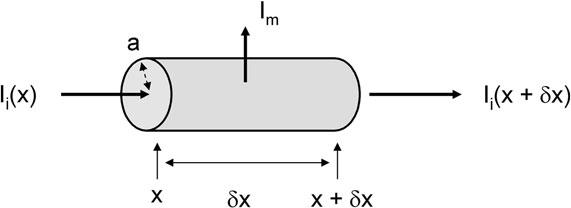
\includegraphics[width=0.8\textwidth]{1218.png}
  \caption{Corriente longitudinal en un axón, con una «caja de pastillas» para examinar el flujo de corriente, incluyendo la corriente de membrana (Basado en [17]).}
  \label{fig:1218}
\end{figure}

\begin{SCfigure}[0.8][htbp]
  \centering
  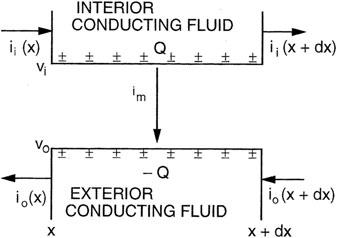
\includegraphics[width=0.55\textwidth]{1219.png}
  \caption{Un modelo más físico para las corrientes del axón mostradas en la Fig. 12.18 (De [17]).}
  \label{fig:1219}
\end{SCfigure}



Aplicaremos la primera ley de Kirchhoff (12.8) a esta construcción y sumaremos todas las corrientes que entran en esta caja de pastillas. Hay flujos de corriente dentro del axón $I_{\text{i}}(x)$ y $-I_{\text{i}}(x + \delta x)$ que entran en la caja de pastillas. También hay un flujo de corriente debido al flujo de iones a través de la membrana celular $I_{\text{m}}$. Diremos que es positiva cuando sale del axón (Fig. 12.18), por lo que $-I_{\text{m}}$ entra en él. El voltaje a través de la membrana celular es $V = q/C_{\text{m}}$, donde $C_{\text{m}}$ es la capacitancia de la membrana. La tasa de cambio temporal del voltaje está relacionada con otra corriente $I_{\text{c}}$ asociada con el cambio de carga en las paredes de la membrana celular
\begin{equation}
\frac{dV}{dt} = \frac{dq/dt}{C_{\text{m}}} = \frac{I_{\text{c}}}{C_{\text{m}}}
\label{eq:12.57}
\end{equation}
o bien
\begin{equation}
I_{\text{c}} = C_{\text{m}} \frac{dV}{dt}.
\label{eq:12.58}
\end{equation}

$I_{\text{c}}$ fluye hacia el exterior, por lo que $-I_{\text{c}} = -C_{\text{m}}(dV/dt)$ fluye hacia el interior del axón. La primera ley de Kirchhoff da
\begin{equation}
I_{\text{i}}(x) - I_{\text{i}}(x + \delta x) - I_{\text{m}} - C_{\text{m}} \frac{dV}{dt} = 0
\label{eq:12.59}
\end{equation}
o
\begin{equation}
I_{\text{i}}(x) - I_{\text{i}}(x + \delta x) - I_{\text{m}} = C_{\text{m}} \frac{dV}{dt}.
\label{eq:12.60}
\end{equation}

Usando $I_{\text{i}}(x + \delta x) \simeq I_{\text{i}}(x) + (dI_{\text{i}}/dx)\delta x$, vemos que $I_{\text{i}}(x) - I_{\text{i}}(x + \delta x) \simeq -(dI_{\text{i}}/dx)\delta x$ y esta ecuación se convierte en
\begin{equation}
-\frac{dI_{\text{i}}}{dx} \delta x - I_{\text{m}} = C_{\text{m}} \frac{dV}{dt}.
\label{eq:12.61}
\end{equation}

Usando la ley de Ohm, la caída de voltaje a través de la caja de pastillas es
\begin{equation}
V(x) - V(x + \delta x) = I_{\text{i}}(x) r_{\text{i}}(\delta x),
\label{eq:12.62}
\end{equation}
donde la resistencia es $R_{\text{i}} = r_{\text{i}}\delta x$. Como $V(x + \delta x) \simeq V(x) + (dV/dx)\delta x$, vemos que $V(x) - (V(x) + (dV/dx)\delta x) \simeq I_{\text{i}}(x) r_{\text{i}}(\delta x)$ o bien
\begin{equation}
I_{\text{i}}(x) = -\frac{1}{r_{\text{i}}} \frac{dV}{dx}.
\label{eq:12.63}
\end{equation}

Tomando la primera derivada de ambos lados se obtiene $dI_{\text{i}}/dx = -(1/r_{\text{i}})d^2V/dx^2$, y la ecuación (12.61) se convierte en
\begin{equation}
\frac{1}{r_{\text{i}}} \frac{d^2V}{dx^2} (\delta x) - I_{\text{m}} = C_{\text{m}} \frac{dV}{dt}.
\label{eq:12.64}
\end{equation}

Dividiendo ambos lados por el área de la superficie de la membrana, que es $(2\pi a)(\delta x)$, se obtiene
\begin{equation}
\frac{1}{2\pi a r_{\text{i}}} \frac{d^2V}{dx^2} - \frac{I_{\text{m}}}{(2\pi a)\delta x} = \frac{C_{\text{m}}}{2\pi a(\delta x)} \frac{dV}{dt}.
\label{eq:12.65}
\end{equation}

Definiendo la densidad de corriente de la membrana (corriente de membrana por unidad de área) como $J_{\text{m}} = I_{\text{m}}/(2\pi a(\delta x))$ y la capacitancia de la membrana por unidad de área expresada como $c_{\text{m}} = C_{\text{m}}/(2\pi a(\delta x))$, esto se convierte en
\begin{equation}
\frac{1}{2\pi a r_{\text{i}}} \frac{d^2V}{dx^2} - J_{\text{m}} = c_{\text{m}} \frac{dV}{dt}
\label{eq:12.66}
\end{equation}
o bien
\begin{equation}
c_{\text{m}} \frac{\partial V(x, t)}{\partial t} = -J_{\text{m}} + \frac{1}{2\pi a r_{\text{i}}} \frac{\partial^2 V(x, t)}{\partial x^2}.
\label{eq:12.67}
\end{equation}

Esto ahora ha sido expresado (correctamente) en términos de derivadas parciales con respecto a $t$ y $x$, lo que significa que las derivadas se toman con respecto a $t$ y $x$, respectivamente, tratando a $x$ y $t$ como constantes. Además, el voltaje se escribe explícitamente como una función de $x$ y $t$.

¿Cómo tratamos el transporte activo de carga a través de la membrana? Modelamos la corriente de la membrana como $g_i(V - V_i)$ para cada ion, siendo $g_i$ la conductancia por unidad de área y $V_i$ un voltaje característico, los cuales son parámetros para el ion específico. La corriente total de la membrana es
\begin{equation}
J_{\text{m}} = \sum_{i} g_i(V - V_i) = g_{\text{Na}}(V - V_{\text{Na}}) + g_{\text{K}}(V - V_{\text{K}}) + g_{\text{L}}(V - V_{\text{L}}),
\label{eq:12.68}
\end{equation}
donde hemos incluido la conducción por iones de $\text{Na}^+$ y $\text{K}^+$ y por otros iones (fuga, L). Este modelo de Hodgkin-Huxley se representa en la Fig. 12.20. Así encontramos
\begin{equation}
c_{\text{m}} \frac{\partial V(x, t)}{\partial t} = -\sum_{i} g_i(V(x, t) - V_i) + \frac{1}{2\pi a r_{\text{i}}} \frac{\partial^2 V(x, t)}{\partial x^2}
\label{eq:12.69}
\end{equation}
o para un solo ion
\begin{equation}
c_{\text{m}} \frac{\partial V(x, t)}{\partial t} = -g_i(V(x, t) - V_i) + \frac{1}{2\pi a r_{\text{i}}} \frac{\partial^2 V(x, t)}{\partial x^2}.
\label{eq:12.70}
\end{equation}

\begin{SCfigure}[0.8][htbp]
  \centering
  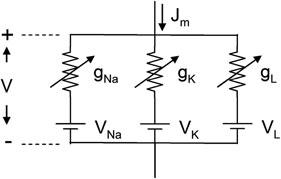
\includegraphics[width=0.55\textwidth]{1220.png}
  \caption{Circuito equivalente del modelo de Hodgkin-Huxley de la corriente de membrana, con resistencias variables $g_i$ y fuentes de voltaje $V_i$ (Basado en [17]).}
  \label{fig:1220}
\end{SCfigure}



Esta última ecuación se conoce como la ecuación del cable o de los telegrafistas porque también describe la propagación de señales eléctricas a lo largo de cables largos, como los cables submarinos, así como la propagación de tales señales a lo largo de los axones en las neuronas. Recuerde que aunque la perturbación de voltaje se propaga a largas distancias, las cargas se mueven muy poco y, de hecho, se mueven esencialmente solo a través de la pared de la membrana, que es perpendicular a la dirección de propagación de la onda. (Por cierto, John Carew Eccles, Alan Lloyd Hodgkin y Andrew Fielding Huxley compartieron el Premio Nobel de Fisiología o Medicina en 1963 por sus descubrimientos sobre los mecanismos iónicos implicados en la excitación e inhibición en las porciones periférica y central de la membrana de la célula nerviosa, que forman parte de este modelo de Hodgkin-Huxley).

Cuando esta onda se propaga a una velocidad $u$, viaja como un pulso (Fig. 12.21) con una forma invariable que tiene $x - ut$ constante. (Véase la discusión sobre la propagación de ondas sonoras en el Cap. 10). Se puede demostrar entonces que $\partial^2 V/\partial t^2 = u^2 \partial^2 V/\partial x^2$ o $\partial^2 V/\partial x^2 = (1/u^2)\partial^2 V/\partial t^2$ y, por lo tanto, la ecuación (12.70) se puede escribir únicamente en términos de derivadas con respecto al tiempo. Incluyendo los tres iones, vemos que:
\begin{equation}
\frac{1}{2\pi a r_{\text{i}} u^2} \frac{\partial^2 V}{\partial t^2} - c_{\text{m}} \frac{\partial V}{\partial t} = g_{\text{Na}}(V - V_{\text{Na}}) + g_{\text{K}}(V - V_{\text{K}}) + g_{\text{L}}(V - V_{\text{L}})
\label{eq:12.71}
\end{equation}
con las propiedades típicas de las neuronas dadas en la Tabla 12.5. Se pueden encontrar más detalles en [17, 18, 23].

\begin{SCfigure}[1.0][htbp]
  \centering
  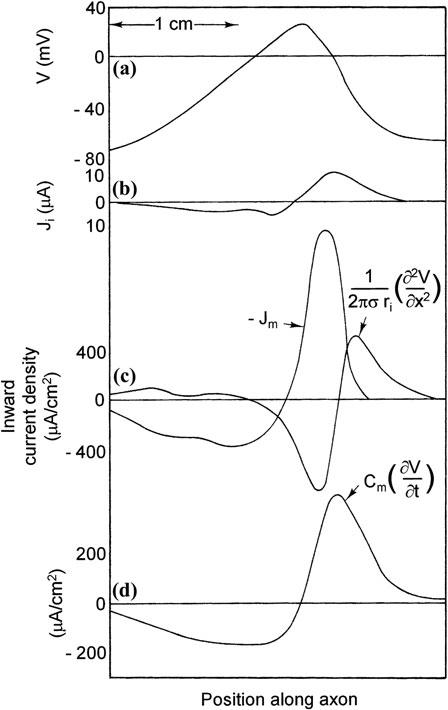
\includegraphics[width=0.45\textwidth]{1221.png}
  \caption{Una instantánea de a) el voltaje y b) la corriente del axón del pulso que se propaga a lo largo de un axón; c) las densidades de corriente correspondientes a los dos términos en el lado derecho de (12.67); d) la corriente que carga o descarga la membrana. Todos están calculados usando (12.67) (De [17]).}
  \label{fig:1221}
\end{SCfigure}



\subsection*{Velocidad de propagación de los potenciales de acción}

Estas ecuaciones deben resolverse numéricamente. Aún así, podemos obtener cierta comprensión sobre la velocidad de estas señales eléctricas a lo largo del axón mediante el uso de un método analítico. Usando (12.47), (12.50) y (12.54), podemos reorganizar (12.70) para obtener
\begin{equation}
\lambda^2 \frac{\partial^2 V(x, t)}{\partial x^2} - V(x, t) - \tau \frac{\partial V(x, t)}{\partial t} = -V_i,
\label{eq:12.72}
\end{equation}
donde
\begin{equation}
\lambda = \sqrt{\frac{1}{2\pi a r_{\text{i}} g_i}} = \sqrt{\frac{a b \rho_{\text{m}}}{2 \rho_{\text{i}}}}
\label{eq:12.73}
\end{equation}
y
\begin{equation}
\tau = \frac{c_{\text{m}}}{g_i} = \kappa \varepsilon_0 \rho_{\text{m}}.
\label{eq:12.74}
\end{equation}

Vemos que $\lambda$ tiene unidades de distancia y $\tau$ tiene unidades de tiempo en (12.72), por lo que no es descabellado pensar que la velocidad de conducción $u$ es aproximadamente
\begin{equation}
u \sim \frac{\lambda}{\tau} = \sqrt{\frac{a b}{2 \rho_{\text{i}} \rho_{\text{m}}}} \frac{1}{\kappa \varepsilon_0}.
\label{eq:12.75}
\end{equation}

Para un axón no mielinizado, $b \approx 6\,\text{nm}$ y, por lo tanto, usando los parámetros de la Tabla 12.5, encontramos
\begin{equation}
u_{\text{unmyelinated}} \sim 0.27\sqrt{a},
\label{eq:12.76}
\end{equation}
donde $u$ está en m/s y $a$ está en $\mu$m. Esto es aproximadamente $7$ veces más lento de lo observado, a saber, $1.8\sqrt{a}$.

Para un axón mielinizado, $b \approx 0.4a$, por lo que $\lambda = 1\,350a$ y
\begin{equation}
u_{\text{myelinated}} \sim 2.2a,
\label{eq:12.77}
\end{equation}
lo cual es nuevamente unas $7$ veces más lento de lo observado, a saber, $17a$. No se espera que este modelo de conducción con una conducción tipo Hodgkin-Huxley a través de la membrana sea muy preciso porque, a diferencia del de la membrana desnuda, la conducción de la vaina de mielina es independiente del voltaje. Por lo tanto, la propagación ocurre en la región de la vaina con este término y hay cierta atenuación hasta que la señal llega al siguiente nodo de Ranvier. La señal se regenera en esta membrana libre de vaina y luego se propaga hasta la siguiente etapa de regeneración. Si en su lugar asumiéramos en el modelo de conducción en axones mielinizados que la velocidad de conducción es $u_{\text{myelinated}} \sim D/\tau$, donde $D \approx 280a$ es la distancia entre los nodos de Ranvier, la velocidad de conducción del modelo sería
\begin{equation}
u_{\text{myelinated}} \sim 0.45a,
\label{eq:12.78}
\end{equation}
lo que es aproximadamente $40$ veces más lento que las observaciones.

La velocidad de la conducción nerviosa se puede medir aplicando un pulso de voltaje estimulante en un lugar del cuerpo y utilizando electrodos para detectar el retraso temporal en el pulso propagado en otro lugar del cuerpo, como se ve en la Fig. 12.22 [4].

\begin{figure}[htbp]
  \centering
  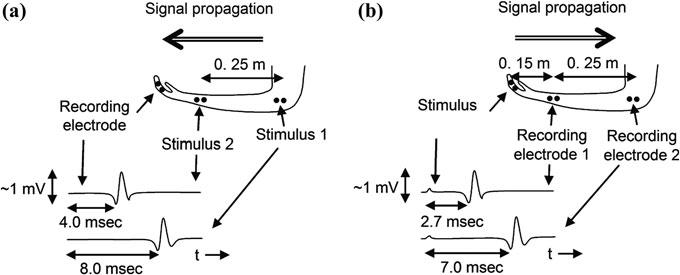
\includegraphics[width=0.8\textwidth]{1222.png}
  \caption{Medición de la velocidad de conducción a lo largo del antebrazo y la mano de a) un nervio motor y b) un nervio sensorial, junto con las señales de EMG asociadas. La velocidad de conducción del nervio motor en (a) es $62.5\,\text{m/s}$, y la velocidad de conducción del nervio sensorial en (b) es $58.1\,\text{m/s}$ (ver Problema 12.18) (Basado en [4]).}
  \label{fig:1222}
\end{figure}



\subsection*{Dispersión pasiva}

Cuando los voltajes están por debajo del umbral de $\sim -55\,\text{mV}$, la perturbación de voltaje del potencial graduado se atenúa a lo largo del axón y en el tiempo. Podemos usar este modelo para entender esto. Esto es equivalente al modelo de circuito distribuido en la Fig. 12.17.

\textbf{Caso especial: Solo resistencia, sin capacitancia, cable infinitamente largo.} Si se desprecia la capacitancia de la membrana en el modelo ($c_{\text{m}} = 0$ y, por tanto, $\tau = 0$), entonces (12.72) se convierte en
\begin{equation}
\lambda^2 \frac{d^2 V(x)}{dx^2} - V(x) = -V_i
\label{eq:12.79}
\end{equation}
y $V$ no depende del tiempo. Si en, digamos, $x = 0$, el voltaje se mantiene en $V = V_i + V_0$, la solución es
\begin{equation}
V(x) = V_i + V_0 \exp(-x/\lambda) \quad \text{para } x > 0
\label{eq:12.80}
\end{equation}
\begin{equation}
V(x) = V_i + V_0 \exp(+x/\lambda) \quad \text{para } x < 0,
\label{eq:12.81}
\end{equation}

lo cual se puede demostrar por sustitución. Esto significa que la perturbación subumbral se atenúa a lo largo de una distancia característica $\lambda$, como se ve en la Fig. 12.23.

\begin{SCfigure}[0.8][htbp]
  \centering
  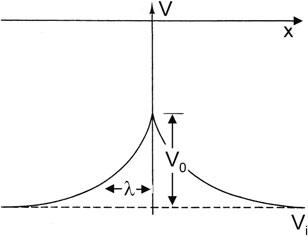
\includegraphics[width=0.55\textwidth]{1223.png}
  \caption{Sin capacitancia de membrana del axón, una perturbación de voltaje se atenúa a lo largo de una distancia característica $\lambda$ (De [17]).}
  \label{fig:1223}
\end{SCfigure}



\textbf{Caso especial: Solo resistencia, sin capacitancia, cable de longitud finita.} Si el cable es semiinfinito o de longitud finita, la solución de (12.79) debe modificarse [26]. Tales soluciones se muestran en la Fig. 12.24 y se examinan más a fondo en el Problema 12.24 (para $V_i = 0$). De particular importancia para un cable de longitud finita es exactamente cómo termina el axón en cada extremo, es decir, las condiciones de contorno. Usualmente estas condiciones de contorno se especifican dando el voltaje $V$ o el flujo de corriente (que es proporcional a $dV/dx$) en el extremo del cable del axón.

\begin{figure}[htbp]
  \centering
  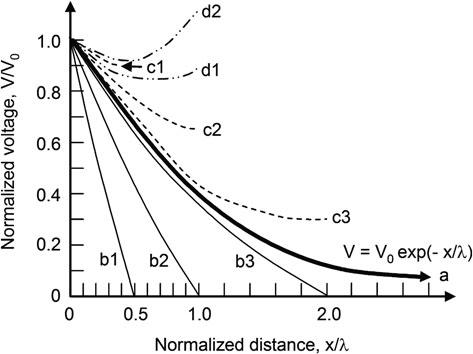
\includegraphics[width=0.7\textwidth]{1224.png}
  \caption{Soluciones en estado estacionario para (12.79) para a) un cable semiinfinito y b)--d) cables de longitud finita $L$ con diferentes condiciones de contorno al final, con distancia característica $\lambda$ y $V = V_0$ en $x = 0$. Para las curvas (b1)--(b3), $V(L) = 0$ (voltaje fijado a cero), para $L = 0.5\lambda$, $\lambda$ y $2.0\lambda$. Para las curvas (c1)--(c3), $dV/dx = 0$ (corriente fijada a cero) en $x = L$, para $L = 0.5\lambda$, $\lambda$ y $2.0\lambda$. Para las curvas (d1) y (d2), el voltaje está fijado a $0.9V_0$ y $1.1V_0$ en $x = L$, para $L = \lambda$. Ver también el Problema 12.24 (Basado en [26]).}
  \label{fig:1224}
\end{figure}



\textbf{Caso especial: Sin resistencia del axoplasma, con capacitancia, cable infinitamente largo.} Si en su lugar la resistencia del axoplasma se establece igual a cero (como por ejemplo al colocar un cable axialmente en el axón), entonces $\lambda^2(\partial^2 V(x, t)/\partial x^2) = 0$ y (12.72) se convierte en
\begin{equation}
\tau \frac{\partial V(x, t)}{\partial t} + V(x, t) = V_i.
\label{eq:12.82}
\end{equation}

(Al igual que en la Fig. 12.17, todavía es posible una resistencia transversal). Si en, digamos, $t = 0$, el voltaje estuviera limitado a $V = V_i + V_0$ y se liberara la limitación, entonces para cualquier $x$
\begin{equation}
V(t) = V_i + V_0 \exp(-t/\tau) \quad \text{para } t > 0.
\label{eq:12.83}
\end{equation}
Nuevamente, esto se puede demostrar por sustitución. Esto significa que la perturbación subumbral se atenúa en un tiempo característico $\tau$.

\textbf{Caso general, cable infinitamente largo.} Podemos encontrar una solución más general sustituyendo una solución de prueba
\begin{equation}
V(x, t) = V_i + w(x, t) \exp(-t/\tau),
\label{eq:12.84}
\end{equation}
en (12.72). Esto conduce a:
\begin{equation}
\frac{\lambda^2}{\tau} \frac{\partial^2 w(x, t)}{\partial x^2} = \frac{\partial w(x, t)}{\partial t}.
\label{eq:12.85}
\end{equation}

Esta es la ecuación de difusión (segunda ley de difusión de Fick, ver (7.66); ver también el Apéndice C). La perturbación $w$ se propaga de manera similar a una gaussiana a lo largo de una distancia $\lambda$ en un tiempo $\tau$, aproximadamente como
\begin{equation}
w(x, t) \propto \exp(-x^2/2D_{\text{diff}}t),
\label{eq:12.86}
\end{equation}
donde la constante de difusión es $D_{\text{diff}} = \lambda^2/\tau$. Esto asume un pico de voltaje inicial en $x = 0$. Usando (12.84), la perturbación de voltaje real se propaga como:
\begin{equation}
V(x, t) - V_i \propto \exp(-x^2/2D_{\text{diff}}t) \exp(-t/\tau),
\label{eq:12.87}
\end{equation}
que tiene una atenuación exponencial global adicional en el tiempo con un tiempo característico $\tau$.

\section[Canales Iónicos, Equilibrio y Sentidos]{Canales iónicos, células ciliadas, equilibrio, gusto y olfato}
\label{sec:12.4}

La sección anterior abordó la conducción de señales en un axón. Igualmente importante es la generación real de señales que luego se conducen a lo largo de un axón hacia el cerebro. Vimos en la sección anterior que el control del flujo de iones a través de la membrana celular ---mediante cambios en la permeabilidad de las membranas a los iones por la apertura o el cierre de canales iónicos--- es importante en esta conducción. También es importante en la generación de señales, como en la percepción sensorial.

Un ejemplo interesante es la excitación de las células ciliadas, que es importante en varias partes del cuerpo. La Figura 12.25 muestra que el «pelo» en una célula ciliada es un haz de cilios compuesto por una serie asimétrica de 20--300 microvellosidades, que se vuelven sucesivamente más grandes en una dirección. Al final del haz a menudo hay un cilio grande, que se llama kinocilio. Cuando el haz de cilios se mueve hacia el kinocilio, el potencial de membrana se despolariza en relación con el potencial de reposo y cuando se aleja de él, la membrana se hiperpolariza, como se ve en la Fig. 12.26. No hay cambio en el potencial de membrana cuando el haz se mueve perpendicularmente a la dirección de las microvellosidades cada vez más grandes. Una posible explicación para esta despolarización es que los canales de iones positivos de $\text{Na}^+$ se abren cuando el haz de cilios se desplaza hacia el kinocilio. La respuesta elástica de la célula ciliada proviene de las propias microvellosidades, de los elementos elásticos (resortes de compuerta) que tiran de los canales iónicos y de los propios canales. La respuesta del pelo a las fuerzas se discutió en el Cap. 10 (texto y Problema 10.55).

\begin{figure}[htbp]
  \centering
  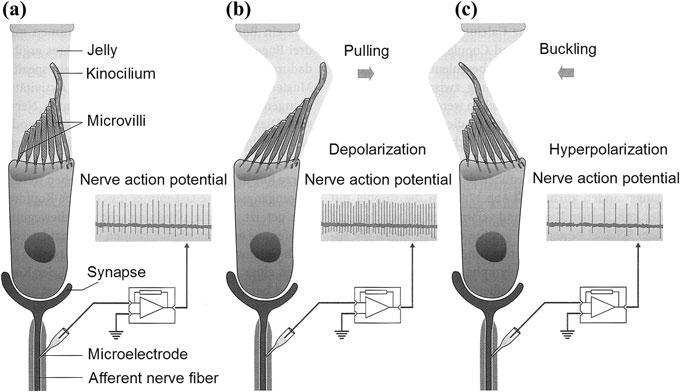
\includegraphics[width=0.8\textwidth]{1225.png}
  \caption{En un mecanismo de respuesta de la célula ciliada, el haz de cilios se mueve hacia el kinocilio (el cilio con la esfera) abriendo canales que son permeables al $\text{Na}^+$ (lo que constituye la despolarización), como se muestra en (b). La actividad en reposo se observa en (a) y la hiperpolarización en (c). a) Estado de reposo. b) Activación. c) Inhibición (De [30]).}
  \label{fig:1225}
\end{figure}

\begin{SCfigure}[0.9][htbp]
  \centering
  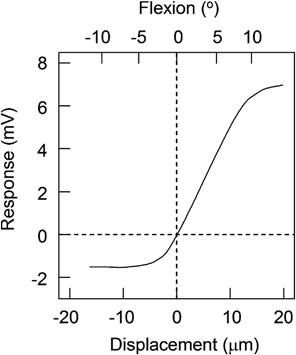
\includegraphics[width=0.5\textwidth]{1226.png}
  \caption{Potencial de membrana frente al desplazamiento del cilio (en posición y ángulo). Los desplazamientos positivos son hacia el kinocilio (Basado en [10, 20]).}
  \label{fig:1226}
\end{SCfigure}



Estas células ciliadas son importantes en el oído, ya que contribuyen tanto a la generación de señales auditivas en la cóclea que viajan al cerebro para permitir la audición, como al sistema vestibular en el oído que nos ayuda a mantener el sentido del equilibrio. Cada oído tiene tres canales semicirculares que son aproximadamente ortogonales entre sí, los cuales nos proporcionan el sentido del equilibrio al detectar el movimiento del fluido en su interior. La Figura 12.27 muestra cómo las células ciliadas detectan uno de estos movimientos, el de girar la cabeza hacia la derecha. Esto es en el sentido de las agujas del reloj visto desde arriba, como en la figura. El fluido en los dos canales semicirculares horizontales representados se retrasa con respecto a este movimiento (primera ley de Newton), por lo que se mueve en sentido contrario a las agujas del reloj en relación con las células ciliadas. Esto provoca una despolarización de las células ciliadas en el oído derecho y una hiperpolarización de las células ciliadas en el oído izquierdo. Estos canales semicirculares contienen células ciliadas bañadas por un fluido, la endolinfa, que tiene altas concentraciones de $\text{K}^+$ y bajas concentraciones de $\text{Na}^+$ y $\text{Ca}^{2+}$. Por consiguiente, cuando las células ciliadas son estimuladas, el $\text{K}^+$ entra en la célula a través de los canales durante esta despolarización. Las células ciliadas de la cóclea también están bañadas por este fluido endolinfático en la rampa media (scala media), por lo que el control de los canales de iones $\text{K}^+$ por parte de los haces de cilios también es importante en la transducción auditiva (donde la transducción es la conversión de un tipo de señal o estímulo en otro por parte de una célula, que en este caso es la conversión del sonido en una señal eléctrica). (El fluido de la perilinfa en la rampa vestibular y en la rampa timpánica es rico en $\text{Na}^+$ y pobre en $\text{K}^+$, al igual que la sangre y el líquido cefalorraquídeo).

\begin{figure}[htbp]
  \centering
  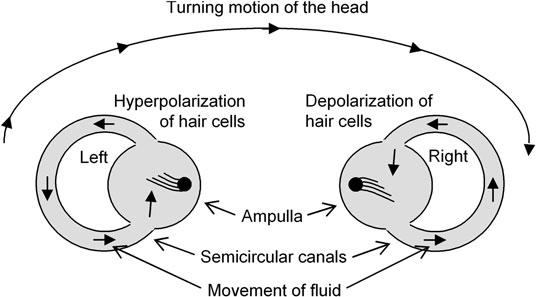
\includegraphics[width=0.8\textwidth]{1227.png}
  \caption{El sentido del equilibrio se observa al examinar el par de canales semicirculares horizontales, mirando la cabeza desde arriba. Cuando se gira la cabeza en el sentido de las agujas del reloj, se produce un movimiento en sentido contrario a las agujas del reloj del fluido coclear que despolariza las células ciliadas en el canal semicircular del oído derecho e hiperpolariza las del oído izquierdo (Basado en [10]).}
  \label{fig:1227}
\end{figure}



Las señales que nos ayudan a mantener el equilibrio provienen de los canales semicirculares del oído interno y de señales visuales. Con el envejecimiento, las personas pierden el equilibrio más fácilmente debido a que la primera vía no funciona bien; las señales visuales se vuelven entonces aún más necesarias.

La importancia de las células ciliadas en el sentido del tacto (para la piel con pelo) se discutió en el Cap. 2. El sentido del tacto por los receptores de Merkel, los corpúsculos de Meissner, los cilindros de Ruffini y los corpúsculos de Pacini tanto en la piel sin pelo como con pelo surge de cambios en los canales iónicos causados por la presión aplicada.

Los sensores de las papilas gustativas se encuentran en agrupaciones llamadas botones gustativos en la lengua y otros lugares de la cavidad oral. Existen varios mecanismos que activan los sensores del gusto para lo dulce, agrio, amargo, salado y «umami», todos los cuales implican el control de los canales iónicos de la membrana. (Umami es la palabra japonesa para delicioso. En este contexto, describe el sabor del glutamato monosódico y otros aminoácidos). El conceptualmente más simple es el de la salinidad, que es detectado por un canal de $\text{Na}^+$ que despolariza la célula detectora.

La región de receptores olfatorios en la nariz tiene un área de $\sim 1\text{--}2\,\text{cm}^2$, con unos $\sim 12$ millones de células receptoras. (Hay unos $\sim 4$ mil millones de estas células en un perro pastor alemán). El sentido del olfato se activa mediante neuronas olfatorias, con la apertura de canales iónicos. En muchas de estas neuronas, esto permite que el $\text{Na}^+$ entre en la célula durante la despolarización, lo que induce un aumento en el disparo de potenciales de acción.

\section{Propiedades eléctricas del corazón}
\label{sec:12.5}

La carga total del corazón es cero durante el latido cardíaco, pero existen separaciones dinámicas entre las cargas positivas y negativas. Estas crean un vector de dipolo eléctrico que gira a medida que aumenta y luego disminuye en magnitud durante cada

\begin{SCfigure}[0.8][htbp]
  \centering
  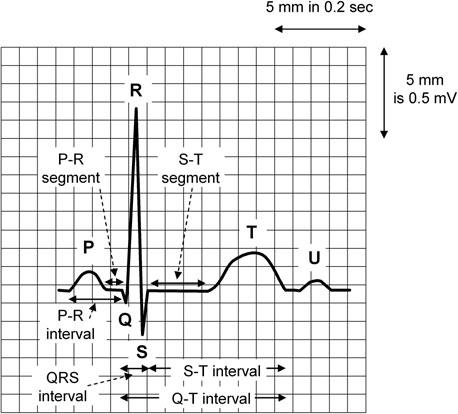
\includegraphics[width=0.55\textwidth]{1228.png}
  \caption{Un electrocardiograma normal (EKG/ECG) que muestra la onda P (despolarización auricular), el complejo QRS (despolarización ventricular) y la onda T (repolarización ventricular) en un solo ciclo cardíaco. Típicamente el registro avanza a $25\text{ mm/s}$ y la intensidad de la señal se grafica como $10\text{ mm/mV}$ (Basado en \cite{23}).}
  \label{fig:1228}
\end{SCfigure}



% Control de Calidad: 35 párrafos origen -> 35 párrafos salida. Mapeo 1:1 verificado. Sin omisiones.

% ---- Bloque 4: temp_cap_12_pag_852_861.tex ----

ciclo cardíaco. El potencial eléctrico en diferentes lugares de la piel, por lo tanto, cambia con el tiempo durante cada ciclo, y esto es lo que se detecta en un electrocardiograma (EKG o ECG). Estas diferencias de potencial son típicamente de $\sim 30$--$500\text{ }\mu\text{V}$. Usualmente se realizan mediciones de EKG escalar de 12 derivaciones, las cuales proporcionan mucha información sobre la evolución del dipolo cardíaco e información suficientemente valiosa sobre posibles anomalías en el corazón. Los EKG vectoriales se realizan con menor frecuencia; pueden proporcionar una visión más completa de la evolución del dipolo cardíaco durante un latido del corazón. En la Fig.~12.28 se muestra un EKG típico.

Desde una perspectiva eléctrica, el corazón puede describirse como un dipolo eléctrico cuya magnitud y dirección varían de manera cíclica, repitiéndose en cada ciclo cardíaco. Al igual que para el axón descrito anteriormente en este capítulo, las posiciones de las cargas en las células del músculo cardíaco cambian durante la despolarización celular en la contracción muscular y la repolarización. Esto constituye un cambio en el momento dipolar eléctrico de la célula individual. Los campos eléctricos debidos a todas estas células del músculo cardíaco se suman para producir variaciones de voltaje en el cuerpo que son detectadas por las sondas del EKG. Los voltajes varían con el tiempo, indicando la despolarización (contracción) de las aurículas derecha e izquierda (llamada onda P), la despolarización (contracción) de los ventrículos derecho e izquierdo durante la sístole (el complejo QRS) y la repolarización de los ventrículos (la onda T); la repolarización de las aurículas queda enmascarada por el complejo QRS. La dependencia temporal puede indicar una activación normal o anormal del músculo cardíaco, y esto podría, en principio, determinarse a partir de la diferencia de voltaje entre dos sondas de EKG. El análisis de los voltajes en varios pares de electrodos proporciona información importante que se utiliza para localizar espacialmente anomalías en diferentes partes del músculo cardíaco, como después de un ataque al corazón. Las sondas del EKG miden el potencial eléctrico (voltaje) justo debajo de la piel. La resistencia a través de la piel no es significativa porque las sondas del EKG se conectan a la piel con un gel de contacto especial.

La diferencia de potencial a través de la membrana celular de la célula del músculo cardíaco cambia durante la despolarización y la subsecuente polarización de los músculos cardíacos auriculares y ventriculares durante cada ciclo, y esto cambia el potencial eléctrico cerca del corazón. Debido a que los tejidos y la sangre del cuerpo contienen iones conductores, tales cambios de potencial causan cambios en las corrientes y los resultados netos afectan el potencial eléctrico muy lejos del corazón. Como tal, el músculo cardíaco puede considerarse como colocado en un conductor de volumen.

¿Por qué cambia este potencial con el tiempo, incluso para una sola célula muscular? Sigamos el movimiento de las cargas durante un ciclo. El campo a través de la membrana celular puede modelarse localmente como un dipolo eléctrico, con cargas positivas y negativas de igual magnitud separadas por una distancia (Fig.~12.1). Las líneas de campo eléctrico se muestran para tal dipolo puntual en la Fig.~12.1.

Una célula de músculo cardíaco polarizada es una serie de tales dipolos, como se muestra en la Fig.~12.29a, con aproximadamente $-70\text{ mV}$ en el interior de la célula en relación con el exterior, alrededor de toda la célula. No se observa potencial (que en realidad es un potencial de línea de base) en el electrodo inmediatamente a la derecha de la célula. A medida que la onda de despolarización se propaga de izquierda a derecha, el potencial a la derecha aumenta y alcanza un máximo cuando la mitad de la célula está despolarizada, como en (c). A medida que la onda de despolarización llega al extremo derecho, este voltaje disminuye a cero como en (e). Esto es similar a la onda PQR en la despolarización ventricular observada en el EKG en la Fig.~12.28. Esto es lo que ocurriría si el potencial a través de la membrana fuera cero después de la despolarización. Debido a que en realidad se vuelve ligeramente positivo, el potencial en (e) debería descender ligeramente hacia valores negativos, como se observa para la onda PQR. Cuando el lado izquierdo se repolariza, el potencial se vuelve negativo y se desarrolla un pulso negativo, como en (f)--(h). Esto es similar al pulso S de repolarización ventricular en la Fig.~12.28, excepto por su signo. A diferencia de lo que ocurre en la Fig.~12.29h, el segundo pico es positivo porque la repolarización del músculo cardíaco procede en la dirección opuesta a la despolarización, como ocurre en la traza inferior. Además, la repolarización es un poco más lenta y más inhomogénea que la despolarización, por lo que el descenso negativo es más amplio (más lento) y tiene una magnitud menor (más superficial) que el primer pico.

\begin{SCfigure}[1.3][htbp]
  \centering
  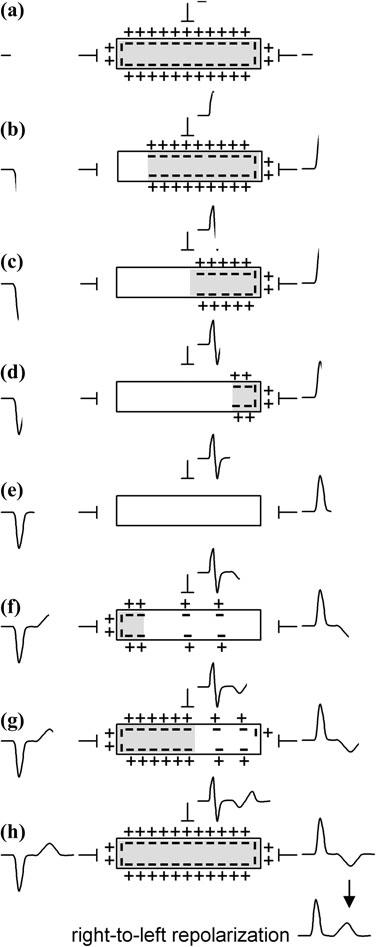
\includegraphics[width=0.35\textwidth]{1229.png}
  \caption{Potencial a la derecha de una tira de miocardio inmersa en un conductor de volumen durante la despolarización (a--e) y repolarización (f--h). La sección polarizada es gris y la sección despolarizada es blanca. Para el músculo cardíaco real, la señal de repolarización es positiva, al igual que la señal de despolarización (Fig.~12.28), debido a que en el corazón humano la repolarización procede en la dirección opuesta a la despolarización, como se muestra en la parte inferior (Basado en \cite{34}).}
  \label{fig:1229}
\end{SCfigure}



La Figura~12.29 también muestra que el potencial es cualitativamente diferente a la izquierda y en la parte superior de la célula durante la despolarización. Esta es la razón por la cual los electrodos de EKG colocados en diferentes posiciones detectan diferentes señales (y pueden proporcionar información diferente). Además, el electrodo colocado a la izquierda en la Fig.~12.29 proporciona el negativo de la señal del colocado a la derecha. (Esto tiene sentido. ¿Por qué?)

Cada uno de los cuatro ciclos de despolarización auricular y ventricular y repolarización auricular y ventricular no ocurre simultáneamente en todo el corazón, y cada uno es detectado por un EKG y puede analizarse por separado. La evolución del dipolo eléctrico cardíaco neto durante la despolarización ventricular (ciclo QRS) se muestra para un corazón normal en la Fig.~12.30.

\begin{figure}[htbp]
  \centering
  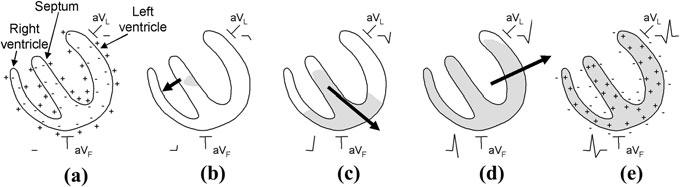
\includegraphics[width=0.8\textwidth]{1230.png}
  \caption{Despolarización ventricular normal registrada por las derivaciones aVL y aVF, que muestra el cambio en magnitud y la rotación en sentido antihorario de la proyección del dipolo cardíaco en el plano frontal (Basado en \cite{21}).}
  \label{fig:1230}
\end{figure}



Claramente, la magnitud y la dirección del dipolo cambian considerablemente durante cada ciclo. Estos cambios son detectados por la colocación exacta de los electrodos de EKG, los cuales pueden proporcionar detalles importantes sobre la función y disfunción cardíacas. La ubicación de las doce derivaciones para un EKG con una persona en decúbito supino (acostada) se describe en la Tabla~12.6. Seis están en las costillas y otras seis están en los brazos y las piernas. Tres de estas últimas tienen dos conductores (bipolares), uno para monitoreo y otro de referencia, mientras que las otras nueve son derivaciones simples (unipolares). Las Figuras~12.31 y 12.32 muestran las nueve ubicaciones de la tabla donde se colocan las 12 derivaciones de EKG. Recuerde que se están midiendo diferencias de voltaje de una derivación a otra.

\begin{table}[h]
  \centering
  \caption{Posición de los electrodos en un EKG. Ver Figs.~12.31 y 12.32.}
  \label{tab:126}
  \small
  \begin{tabularx}{\textwidth}{>{\hsize=0.4\hsize}X >{\hsize=1.6\hsize}X}
    \toprule
    \textbf{Derivación} & \textbf{Posición del electrodo} \\
    \midrule
    \multicolumn{2}{l}{\textbf{Derivaciones estándar de extremidades (Bipolares)}} \\
    I   & Brazo derecho y brazo izquierdo \\
    II  & Brazo derecho y pierna izquierda \\
    III & Brazo izquierdo y pierna izquierda \\
    \midrule
    \multicolumn{2}{l}{\textbf{Derivaciones aumentadas (Unipolares)}} \\
    aVR & Brazo derecho \\
    aVL & Brazo izquierdo \\
    aVF & Pierna izquierda \\
    \midrule
    \multicolumn{2}{l}{\textbf{Derivaciones torácicas (Unipolares)}} \\
    V1  & 4.º espacio intercostal, lado derecho del esternón \\
    V2  & 4.º espacio intercostal, lado izquierdo del esternón \\
    V3  & 5.º espacio intercostal, lado izquierdo (entre V2 y V4) \\
    V4  & 5.º espacio intercostal, lado izquierdo (línea medioclavicular) \\
    V5  & 5.º espacio intercostal, lado izquierdo (línea axilar anterior) \\
    V6  & 5.º espacio intercostal, lado izquierdo (línea medioaxilar) \\
    \bottomrule
  \end{tabularx}
  \begin{flushleft}
    \small Utilizando información de \cite{11}.
  \end{flushleft}
\end{table}

La discusión anterior muestra que el voltaje del EKG es positivo cuando el dipolo cardíaco apunta hacia el (lado positivo de la) derivación del EKG y negativo cuando apunta en dirección opuesta a esta. Esto queda claro en la Fig.~12.1d. La Figura~12.33 muestra las 12 señales de EKG de un corazón normal. La Figura~12.30 muestra la relación entre la colocación efectiva de dos de estas derivaciones bipolares, la evolución del dipolo cardíaco y la señal registrada por estas derivaciones.

\begin{figure}[htbp]
  \centering
  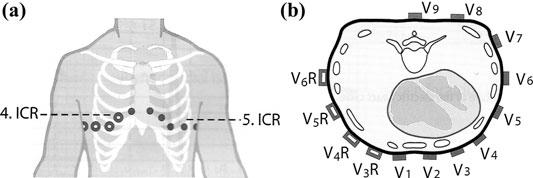
\includegraphics[width=0.8\textwidth]{1231.png}
  \caption{Colocación de los electrodos de EKG unipolares precordiales en el plano horizontal. En los EKG habituales solo se utilizan 6 de las 12 derivaciones en (b), V1--V6 (círculos llenos, en la región etiquetada como 5.ICR (5.º espacio o región intercostal en las costillas) en (a)). Las derivaciones dorsales adicionales V7--V9 se utilizan específicamente para detectar un infarto de miocardio posterior. Las derivaciones precordiales derechas adicionales, V3R--V6R (círculos abiertos, en la región etiquetada como 4.ICR (4.º espacio o región intercostal) en (a)), se utilizan específicamente para detectar un infarto de miocardio del ventrículo derecho (De \cite{13}).}
  \label{fig:1231}
\end{figure}

\begin{figure}[htbp]
  \centering
  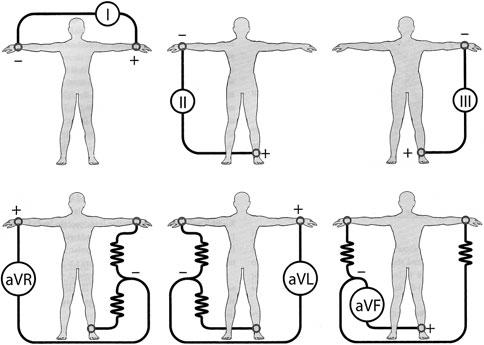
\includegraphics[width=0.7\textwidth]{1232.png}
  \caption{Colocación de las tres derivaciones unipolares y las tres bipolares de las extremidades en el plano frontal. A veces se coloca un electrodo en la pierna derecha (no mostrado) para que sirva como tierra eléctrica (De \cite{13}).}
  \label{fig:1232}
\end{figure}

\begin{figure}[htbp]
  \centering
  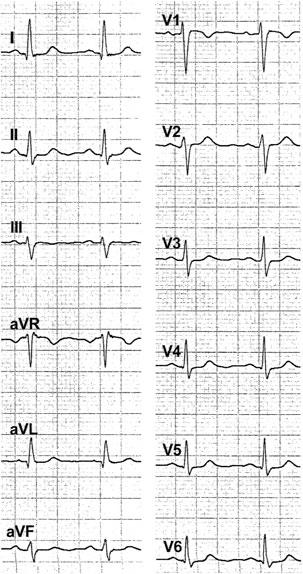
\includegraphics[width=0.4\textwidth]{1233.png}
  \caption{Patrones de EKG normales de los 12 electrodos (De \cite{13}).}
  \label{fig:1233}
\end{figure}

\begin{figure}[htbp]
  \centering
  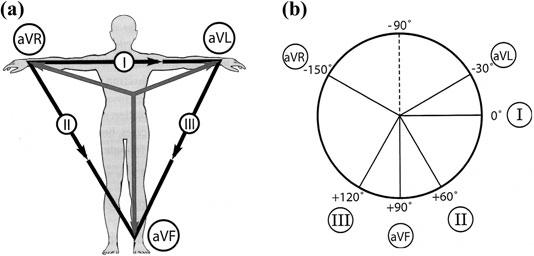
\includegraphics[width=0.8\textwidth]{1234.png}
  \caption{a) Las tres derivaciones I, II y III se organizan como el triángulo de Einthoven. b) Las direcciones efectivas para las seis derivaciones frontales mostradas en (a) se trasladan para formar el sistema de referencia triaxial llamado círculo de Cabrera. La proyección vectorial con signo del dipolo cardíaco sobre estas seis direcciones proporciona la señal de EKG para estas seis derivaciones del plano frontal (De \cite{13}).}
  \label{fig:1234}
\end{figure}



Tres de los electrodos de EKG se colocan en los brazos derecho e izquierdo y en la pierna izquierda, y se monitorean los voltajes a través de los tres pares de estos electrodos (junto con las señales de las otras sondas), los cuales se denominan I ($V_{\text{I}} = V_{\text{left arm}} - V_{\text{right arm}}$), II ($V_{\text{II}} = V_{\text{left leg}} - V_{\text{right arm}}$) y III ($V_{\text{III}} = V_{\text{left leg}} - V_{\text{left arm}}$), como se indica en la Tabla~12.6. Estos tres electrodos actúan como si midieran en los vértices de un triángulo, el cual usualmente se denomina triángulo de Einthoven, como se muestra en la Fig.~12.34a. Debido a que los brazos y las piernas no tienen nuevas fuentes de campos eléctricos y el tejido en cada uno es un conductor, las sondas en los brazos en realidad detectan los mismos voltajes que si se colocaran en sus respectivos hombros, y la sonda en la pierna detecta el mismo voltaje que si se colocara en la parte inferior del torso, cerca de la zona púbica; en consecuencia, el triángulo de Einthoven a veces se representa como este triángulo más pequeño. Utilizando la segunda ley de Kirchhoff, (12.14), $V_{\text{I}} + V_{\text{III}} - V_{\text{II}} = 0$ (el signo menos delante del último potencial indica una convención de signos diferente alrededor del circuito que para los dos primeros) o
\begin{equation}
V_{\text{I}} + V_{\text{III}} = V_{\text{II}}.
\label{eq:12.88}
\end{equation}

El círculo de Cabrera en la Fig.~12.34b muestra la colocación efectiva de las seis derivaciones del plano frontal, y esto se utiliza en la Fig.~12.30.

La Figura~12.34 muestra cómo los dipolos cardíacos momentáneos en tres direcciones diferentes causan diferencias de potencial momentáneas en estos tres pares de electrodos. Una suma apropiada de estos tres voltajes, tal como $V_{\text{I}} + V_{\text{III}} - V_{\text{II}}$, sirve como tierra eléctrica para las mediciones con cada una de las seis sondas del tórax. Además, observe que la diferencia en las señales de las derivaciones aVL y aVF en la Fig.~12.30 debería ser similar a la de la derivación III.

Este EKG puede proporcionar detalles importantes sobre la función y disfunción cardíacas, así como la ubicación de la disfunción. Esto incluye: (1) la frecuencia cardíaca, (2) arritmias, (3) el eje (que indica la dirección y magnitud de la actividad para las contracciones auricular y ventricular), (4) hipertrofia (que es un aumento de la masa muscular ventricular izquierda o derecha), (5) agrandamiento (que es un aumento en el volumen de las cavidades auricular izquierda o derecha) e (6) infarto. En las arritmias, puede haber (a) un ritmo variable, (b) un ritmo que es demasiado rápido (taquicardia, $>100\text{ latidos/min}$; con $>250\text{ latidos/min}$ [aleteo o fibrilación] puede ser potencialmente mortal en los ventrículos) o demasiado lento (bradicardia, $<60\text{ latidos/min}$, excepto que puede ser menor en atletas entrenados), o (c) desviaciones de una relación 1:1 de las contracciones auriculares y ventriculares, como se describe más detalladamente en el Cap.~8.

Durante un infarto de miocardio, parte del músculo cardíaco se daña y, en pocas horas, estas células musculares suelen morir y luego no se despolarizan ni se repolarizan. La ausencia de señales eléctricas de una parte determinada del ventrículo izquierdo se observa en el EKG en la Fig.~12.35. El vector dipolo durante la despolarización apunta en dirección opuesta a la región negra del infarto en el paso 3; si esa región negra estuviera activa, entonces se despolarizaría y el dipolo apuntaría en la dirección opuesta. Esto se observa como una onda Q acentuada. La formación de cicatrices en esta región dañada aún se puede ver después de la recuperación (Fig.~12.36). En general, ondas Q grandes en los registros I y aVL indican un infarto lateral; en los registros V1, V2, V3 o V4, un infarto anterior; y en los registros II, III y aVF, un infarto inferior. Una onda R grande en los registros V1 y V2 indica un infarto posterior.

\begin{figure}[htbp]
  \centering
  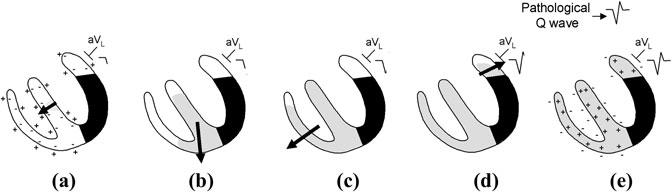
\includegraphics[width=0.8\textwidth]{1235.png}
  \caption{Evolución del dipolo cardíaco durante la despolarización ventricular después de un infarto de miocardio en la pared lateral, junto con el EKG de la derivación aVL. La onda Q más grande de lo normal ocurre porque el sitio del infarto (negro) debería estar despolarizándose y contribuyendo con una señal positiva en (c) (Basado en \cite{21}).}
  \label{fig:1235}
\end{figure}

\begin{figure}[htbp]
  \centering
  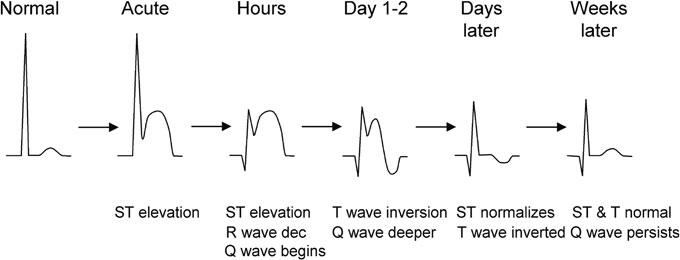
\includegraphics[width=0.8\textwidth]{1236.png}
  \caption{Evolución del EKG durante y después de un infarto agudo de miocardio con onda Q (Basado en \cite{21}).}
  \label{fig:1236}
\end{figure}



La Figura~12.37 muestra los 12 registros de EKG $2\text{ h}$ después de un infarto de miocardio anteroseptal (es decir, uno con características de infartos de miocardio tanto anteriores como septales [interventriculares]) y luego $4\text{ h}$ después de que el infarto ha sido tratado mediante trombolisis (tratamiento para disolver coágulos sanguíneos). No hay una onda Q patológica en este caso, sino ondas ST elevadas a las $2\text{ h}$ y un segmento ST normal $4\text{ h}$ después, aunque todavía se observa una onda T negativa en algunos registros. (Compare ambos con las trazas normales en la Fig.~12.33.)

\begin{figure}[htbp]
  \centering
  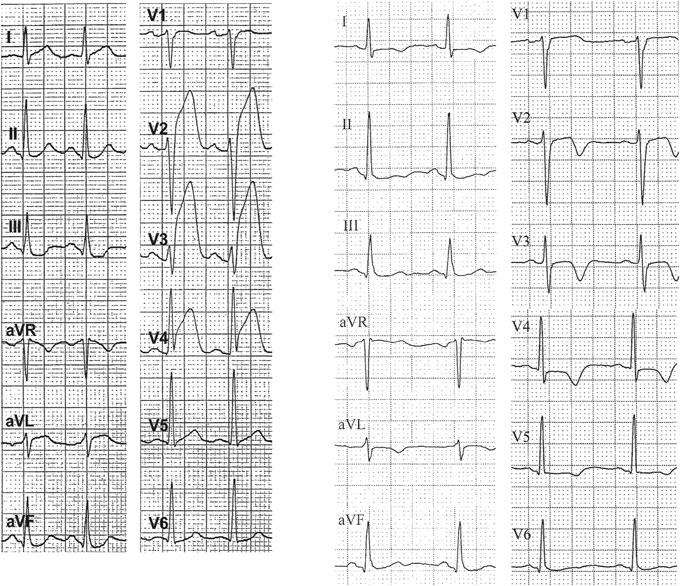
\includegraphics[width=0.7\textwidth]{1237.png}
  \caption{Señales de EKG de las 12 derivaciones (izquierda) $2\text{ h}$ después de un infarto de miocardio anteroseptal y (derecha) $4\text{ h}$ después, después de la trombolisis (De \cite{13}).}
  \label{fig:1237}
\end{figure}

\begin{SCfigure}[0.9][htbp]
  \centering
  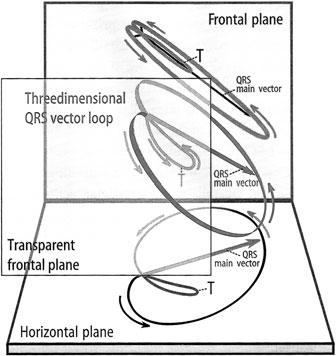
\includegraphics[width=0.5\textwidth]{1238.png}
  \caption{Un vectorcardiograma ventricular que muestra la evolución del vector QRS a lo largo de su lazo, junto con sus proyecciones en los planos frontal y horizontal. La proyección frontal proporciona el EKG del plano frontal derivado de las derivaciones del plano frontal, que necesitan poca corrección; mientras que la proyección horizontal debe corregirse para obtener el EKG escalar obtenido directamente de las derivaciones precordiales (De \cite{13}).}
  \label{fig:1238}
\end{SCfigure}



La información de estas mediciones escalares se puede proyectar sobre diferentes planos corporales y proporcionar información sobre la evolución de los vectores del dipolo cardíaco en un proceso llamado vectorcardiografía. La Figura~12.38 muestra la evolución del vector QRS en un vectorcardiograma y sus proyecciones en los planos frontal y horizontal. Para más información sobre los EKG y el diagnóstico utilizando EKG, consulte \cite{8, 13, 21, 23, 24, 27, 28, 33, 34}.

\section{Señales eléctricas en el cerebro}
\label{sec:12.6}

Las señales eléctricas también son importantes en otras partes del cuerpo y pueden medirse, como se muestra en la Tabla~12.1, tales como los electroencefalogramas (EEG) de las ondas cerebrales en la Fig.~12.39. En contraste con los patrones de EKG muy regulares, la señal de EEG es irregular, pero tiene patrones rítmicos identificables: ondas alfa (frecuencia de $8$--$13\text{ Hz}$; estado despierto, relajado), ondas beta ($14$--$25\text{ Hz}$; vigilia alerta, activación adicional, tensión), ondas theta ($4$--$7\text{ Hz}$, principalmente en niños, también en adultos con estrés emocional y con muchos trastornos cerebrales) y ondas delta ($<3{,}5\text{ Hz}$; sueño profundo) \cite{23}.

\begin{figure}[htbp]
  \centering
  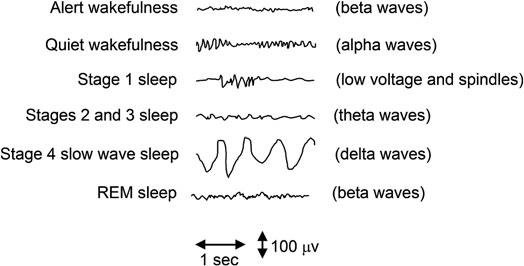
\includegraphics[width=0.8\textwidth]{1239.png}
  \caption{Esquema de los cambios en las ondas cerebrales durante diferentes etapas de la vigilia y el sueño (Basado en \cite{16, 30}).}
  \label{fig:1239}
\end{figure}



\section{Efectos de las descargas eléctricas}
\label{sec:12.7}

Las corrientes eléctricas externas que circulan por el cuerpo pueden causar daños al interferir con el funcionamiento corporal normal ---como al impedir que los músculos esqueléticos y cardíacos, que de otro modo estarían operativos, funcionen normalmente--- y al destruir tejidos por calentamiento térmico (Tabla~12.7). Los músculos son controlados por una serie de impulsos eléctricos enviados por el cerebro. Las corrientes alternas (CA) externas ($60\text{ Hz}$) por encima de unos $10\text{ mA}$ anulan estas señales e impiden que se ejerza control sobre los músculos. Apenas se pueden controlar los músculos a $10\text{ mA}$ y apenas se puede «soltar» un objeto. A corrientes más altas, los músculos quedan bajo control externo, lo que posiblemente provoque dificultades respiratorias y circulatorias. La fibrilación ventricular ocurre entre $100\text{ mA}$ y $4\text{ A}$, y se produce parálisis, junto con quemaduras graves (y la muerte), por encima de $4\text{ A}$. Para descargas débiles, la sensación de descarga varía como la potencia $3{,}5$ del voltaje de $60\text{ Hz}$ aplicado (ley de Stevens~(1.6), Tabla~1.15), por lo que la percepción de una descarga eléctrica es altamente superlineal con el estímulo.

\begin{SCfigure}[1.3][htbp]
\centering
  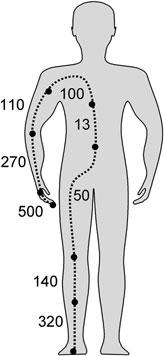
\includegraphics[width=0.35\textwidth]{1240.png}
  \caption{Resistencia de segmentos corporales (en ohmios), ignorando la contribución de la piel. Como se muestra, $500\,\Omega$ es la contribución de un dedo (Basado en \cite{15})}
  \label{fig:12.40}
\end{SCfigure}



\begin{table}[h]
  \centering
  \caption{Efecto de las corrientes (en mA) sobre el cuerpo humano (durante aproximadamente $1\text{ s}$).}
  \label{tab:127}
  \small
  \begin{tabularx}{\textwidth}{>{\hsize=1.8\hsize}X 
                              >{\centering\arraybackslash\hsize=0.6\hsize}X 
                              >{\centering\arraybackslash\hsize=0.6\hsize}X}
    \toprule
    \textbf{Efecto} & \textbf{CC} & \textbf{CA ($60\text{ Hz}$)} \\
    \midrule
    Sensación leve en el punto de contacto & 0,6 & 0,3 \\
    Umbral de percepción & 3,5 & 0,7 \\
    Descarga (shock) & & \\
    -- No dolorosa, sin pérdida del control muscular & 6 & 1,2 \\
    -- Dolorosa, sin pérdida del control muscular & 41 & 6 \\
    -- Dolorosa, umbral de soltar (let-go) & 51 & 10,5 \\
    -- Dolorosa, efectos graves: contracciones musculares, dificultad respiratoria & 60 & 15 \\
    -- Posible fibrilación ventricular (pérdida del ritmo cardíaco normal) & 500 & 100 \\
    \bottomrule
  \end{tabularx}
  \begin{flushleft}
    \small Utilizando datos de \cite{32}. Todos los valores son aproximados.
  \end{flushleft}
\end{table}

% Control de Calidad: 18 párrafos origen -> 18 párrafos salida. Mapeo 1:1 verificado. Sin omisiones.

% ---- Bloque 5: temp_cap_12_pag_862_871.tex ----

La piel es una barrera muy importante para el flujo de corriente ($I$). La resistencia ($R$) a través de la piel seca es de aproximadamente $100\,000\text{--}600\,000\,\Omega$ y a través de la piel húmeda es de solo unos $1000\,\Omega$. Si se supera la barrera de la piel, la resistencia cae (por lo que hay más flujo de corriente por unidad de voltaje, según la ley de Ohm). La Figura~12.40 muestra que la resistencia interna del cuerpo es baja, aproximadamente $400\text{--}600\,\Omega$ de cabeza a pies y $100\,\Omega$ de oreja a oreja. La cantidad de corriente que puede fluir en el cuerpo inducida por una fuente de voltaje ($V$) está limitada por dos factores: (1) la ley de Ohm dice que la corriente será $I = V/R$ y (2) la corriente a veces está limitada por la propia fuente de voltaje.

Asumamos que la barrera de la piel se ha roto, por lo que la resistencia efectiva del cuerpo es de unos $500\,\Omega$. (¡Por favor, no intente esto!). La corriente alterna (CA) de $120\text{ V}$ de un tomacorriente de pared producirá una corriente de $240\text{ mA}$, que es más del doble de la necesaria para causar la muerte por fibrilación ventricular. Los disyuntores normalmente se activan a $15\text{ A}$, por lo que este flujo a través del cuerpo no será interrumpido por el disyuntor. ¿Qué hay de las fuentes de corriente continua (CC)? La corriente inducida por la batería de $9\text{ V}$ que se usa a menudo es de $18\text{ mA}$, lo que puede causar una descarga eléctrica. (Usted puede extraer fácilmente esta corriente de una batería de este tipo). El voltaje a través de una batería de automóvil es de $12\text{ V}$ con $400\text{--}600\text{ A}$ (amperios de arranque), por lo que puede darle una descarga aún peor (Problema~12.5).

\section{Propiedades magnéticas}

Los campos magnéticos en el cuerpo se deben a corrientes eléctricas y son extremadamente débiles. En la Tabla~12.8 se muestran los campos magnéticos típicos en el cuerpo que se pueden medir, y todos son mucho más débiles que el campo magnético de la Tierra de $5 \times 10^{-5}\text{ T}$ ($0.5\text{ Gauss}$). (Para comparar, los campos magnéticos máximos producidos por el ser humano se aproximan a $100\text{ T}$).

\begin{table}[htbp]
\centering
\caption{Amplitud típica de las señales biomagnéticas}
\label{tab:12.8}
\begin{tabularx}{\textwidth}{X c}
\toprule
\textbf{Señal biomagnética} & \textbf{Amplitud típica (pT)} \\
\midrule
Magnetocardiograma (MCG) & 50 \\
MCG fetal & 1\text{--}10 \\
Magnetoencefalograma & 1 \\
Campos evocados & 0.1 \\
Magnetomiograma & 10 \\
Magneto-oculograma & 10 \\
Campo de la Tierra & $50 \times 10^6$ \\
\bottomrule
\end{tabularx}
\addvspace{5pt}
\raggedright\small Con datos de \cite{3}
\end{table}

\subsection{Campo magnético de un axón}

La ley de Biot-Savart determina el campo magnético a partir de corrientes. Considere una corriente continua $I$ que fluye a lo largo del eje $z$ infinitamente largo. Utilizando la ley de Biot-Savart, se puede demostrar que a una distancia $R$, el campo magnético $\vec{\mathbf{B}}$ tiene una magnitud
\begin{equation}
B = \frac{\mu_0 I}{2\pi R}
\label{eq:12.89}
\end{equation}
y está en la dirección radial, de acuerdo con la regla de la mano derecha habitual.

Este análisis no se aplica exactamente a las señales a lo largo de un axón neuronal. Un pulso de voltaje que viaja a lo largo de un axón es un pulso y no una corriente continua. Se encuentra en un medio que es bastante conductor. Además, hay varias direcciones del flujo de corriente: a lo largo del axón, transversal a la membrana, etc. Aun así, estimemos la intensidad del campo justo cuando pasa el pulso, y modelémoslo como una corriente continua. La corriente a lo largo del axón es la más importante. Utilizando (12.63), $I_i(x) = -(1/r_i) dV/dx$, estimamos que la magnitud de esta corriente es
\begin{equation}
I \sim \frac{1}{r_i} \frac{V}{\lambda}.
\label{eq:12.90}
\end{equation}
Por lo tanto, la magnitud del campo magnético a $1\text{ mm}$ de distancia del axón es aproximadamente
\begin{equation}
B \sim \frac{\mu_0 V}{2\pi R r_i \lambda}
\label{eq:12.91}
\end{equation}
\begin{equation}
= \frac{(4\pi \times 10^{-7}\text{ T}\cdot\text{m/A})(0.1\text{ V})}{2\pi (0.001\text{ m})(6.4 \times 10^9\,\Omega\text{/m})(3.8 \times 10^{-4}\text{ m})} = 8\text{ pT},
\label{eq:12.92}
\end{equation}
con $\lambda = 3.8 \times 10^{-4}\text{ m}$. Este valor es consistente con los valores bajos de la Tabla~12.8. (Esta estimación es razonable a pesar de que algunas de las suposiciones no son perfectas).

\subsection{Sentido magnético}

Los seres humanos (aparentemente) no pueden sentir los campos magnéticos, pero los campos magnéticos sí ayudan a varios animales a percibir la dirección (como con una brújula) y/o la ubicación debido a la presencia de partículas de magnetita ($\text{Fe}_3\text{O}_4$) de $50\text{ nm}$ de diámetro en sus cuerpos. (Estas partículas a veces están organizadas en cadenas). Por ejemplo, este sentido magnético es muy fuerte en las palomas, que tienen una sensibilidad de $10\text{--}20\text{ nT}$, y en los delfines, que tienen una sensibilidad de $<2\text{ }\mu\text{T}$ \cite{1}. El mecanismo del sentido magnético puede involucrar un torque inducido en este sistema de partículas por el campo, y esto a su vez puede inducir un torque en los filamentos intracelulares; este movimiento de los filamentos activa una neurona sensorial. (Los campos eléctricos inducen un torque en un dipolo eléctrico, como se ve fácilmente al examinar las fuerzas de Coulomb sobre las cargas individuales en el dipolo eléctrico. De manera similar, los campos magnéticos inducen un torque en un momento magnético. Esta analogía es válida a pesar de que no existen cargas magnéticas).

\section{Ondas electromagnéticas}

Las ondas de radio, las microondas, la radiación infrarroja, la luz visible, la luz ultravioleta, los rayos X y los rayos gamma son todas ondas electromagnéticas. Cada una se propaga a la misma velocidad de la luz $c$ en el vacío. Cada una tiene una frecuencia de oscilación $\nu$ y una longitud de onda $\lambda$ relacionadas por $c = \lambda\nu$ (11.2). Para cada una, esta oscilación consiste en campos eléctricos y magnéticos que oscilan sinusoidalmente en fase en el vacío. Difieren solo en su frecuencia (y, en consecuencia, en su longitud de onda), la cual aumenta (a medida que su longitud de onda disminuye) al pasar de uno de estos regímenes al siguiente. Discutimos la luz visible en detalle en el Cap.~11.

La penetración de la radiación electromagnética a través del cuerpo es a veces de interés. El factor de atenuación para dicha radiación graficado en la Fig.~12.41 es $\alpha_{\text{light}}$ de la ley de Beer, (10.18),
\begin{equation}
I(z) = I(z = 0) \exp(-\alpha_{\text{light}} z).
\label{eq:12.93}
\end{equation}
La atenuación consiste en pérdidas por absorción y dispersión, y es claramente muy dependiente de la frecuencia. Esta figura muestra tendencias, pero no todos los detalles. Por ejemplo, el factor de atenuación en las microondas se debe a procesos no resonantes. El cuerpo absorbe la radiación de microondas a $2.45\text{ GHz}$ utilizada en los hornos de microondas con mucha más fuerza de lo indicado allí debido a la fuerte absorción resonante del agua a esta frecuencia. (Esta es la razón por la que se utiliza esta frecuencia en los hornos de microondas).

\section{Resumen}

Los procesos eléctricos son esenciales para el funcionamiento del cuerpo y han demostrado ser muy importantes en el diagnóstico médico. La conducción eléctrica es importante en la mayoría de las partes del cuerpo. Los modelos de propagación de señales eléctricas en los nervios pueden explicar la base física de tal vez el mecanismo de regulación más importante del cuerpo. Los procesos eléctricos son parte integral del funcionamiento celular, incluyendo la física de las membranas celulares. La naturaleza eléctrica del corazón ha llevado al uso de los ECG como una herramienta de diagnóstico que se puede interpretar mediante modelos simples de la naturaleza dipolar del corazón. Las señales eléctricas en otras partes del cuerpo también se utilizan en el diagnóstico. Las señales magnéticas que ocurren naturalmente son relativamente menos importantes en el cuerpo humano.

\begin{figure}[htbp]
\centering
  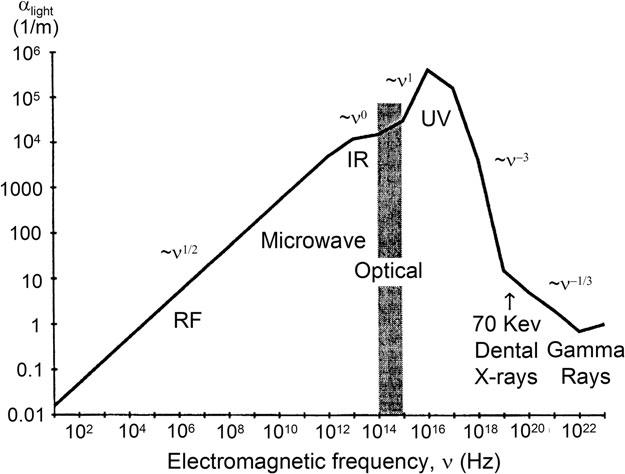
\includegraphics[width=0.7\textwidth]{1241.png}
  \caption{Atenuación de la radiación electromagnética en tejido humano, debido a la absorción y dispersión (De \cite{12}. Cortesía de Robert A. Freitas Jr., Nanomedicine, Vol. 1 (1999), \protect\url{http://www.nanomedicine.com})}
  \label{fig:12.41}
\end{figure}



\section*{Problemas}

\subsection*{Conductancia, transmisión y potenciales}

\noindent \textbf{12.1} Utilice la Tabla~12.4 para comparar la conductividad en una célula y en la sangre.

\noindent \textbf{12.2} Estime la resistencia eléctrica de la sangre en una arteria de $50\text{ cm}$ de longitud y $3\text{ mm}$ de diámetro.

\noindent \textbf{12.3} Existen dos relaciones comunes para la resistividad de la sangre en función del hematocrito, $\text{Hct}$: $\rho = 0.537 \exp(0.025\text{Hct})$ y $\rho = 0.586(1 + 0.0125\text{Hct})/(1 - 0.01\text{Hct})$, la cual se conoce como la ecuación de Maxwell-Fricke \cite{23}. ¿Cómo difieren en el rango de $\text{Hct}$ de $10\text{--}60\%$, y específicamente en el valor normal de $45\%$?

\noindent \textbf{12.4} Durante un accidente, una corriente alterna de $120\text{ V}$ de un tomacorriente de pared conecta su cuerpo a la tierra eléctrica, de mano a mano: \\
(a) Si la resistencia a través del cuerpo es de $500\,\Omega$, ¿cuál es el flujo de corriente? \\
(b) ¿Es esto peligroso? \\
(c) Si la región de mano a mano se puede modelar como un cilindro de diámetro constante (igual al diámetro de la parte superior del brazo) y longitud (desde la punta del dedo hasta la punta del dedo) de su propio cuerpo, y se asume que todo el material es uniforme, estime la resistividad eléctrica del tejido corporal. \\
(d) ¿Cuánta potencia se disipa en esta sección? (Calcule tanto la potencia total como la potencia por unidad de volumen). (Recuerde que la potencia disipada es $P = I V$ y la ley de Ohm es $V = I R$. Asuma aquí y a continuación que la potencia es la misma que la de una fuente de voltaje de CC). \\
(e) ¿Cuál es la capacidad calorífica de esta sección cilíndrica? Asuma el calor específico promedio del cuerpo. \\
(f) Ignorando el flujo de calor, ¿cuánto aumentaría la temperatura de esta sección por unidad de tiempo? \\
(g) ¿Cuánto tiempo tomaría desnaturalizar las proteínas en esta sección cilíndrica? (Ver la información provista en el Cap.~13).

\noindent \textbf{12.5} Compare la cantidad de corriente que se podría extraer de una batería de automóvil en una descarga eléctrica con la cantidad máxima de corriente que se podría extraer de ella. ¿Qué significa esto? ¿Por qué la descarga es peor que la de una batería de $9\text{ V}$?

\noindent \textbf{12.6} ¿Qué rangos de radiación electromagnética pueden penetrar a través de su (a) párpado, (b) dedo y (c) pecho?

\noindent \textbf{12.7} Un ion de masa $m$ y carga $q$ se mueve a una velocidad $v$ bajo la influencia de un campo eléctrico $E$. Sufre una fuerza de arrastre que relaja su velocidad con un tiempo característico $\tau$: \\
(a) Demuestre que el equilibrio de fuerzas sobre la carga da: $m \frac{dv}{dt} = -\frac{m v}{\tau} + qE$. \\
(b) Demuestre que en estado estacionario, el ion se mueve a la velocidad de deriva (que en realidad es la rapidez de deriva aquí), $v_{\text{drift}} = \frac{q E \tau}{m} = \mu E$, donde $\mu = \frac{q \tau}{m}$ se denomina movilidad.

\noindent \textbf{12.8} (\textbf{problema avanzado}) Demuestre que el potencial de una carga $Ze$ blindada por cargas móviles viene dado por $V(r) = \frac{Ze}{4\pi\epsilon_0\epsilon r} \exp(-\kappa r)$, donde $\kappa = \sqrt{\frac{e^2}{\epsilon_0\epsilon k_B T} \sum_i Z_i^2 n_{i,0}}$. Haga esto sustituyendo esta solución para $V(r)$ en la ecuación de Poisson-Boltzmann \eqref{eq:12.41}, que puede expresarse en tres dimensiones como:
\begin{equation}
\frac{1}{r} \frac{d^2(rV)}{dr^2} = -\frac{1}{\epsilon_0 \epsilon} \sum_i Z_i e n_{i,0} \exp\left(-\frac{Z_i e V}{k_B T}\right)
\label{eq:12.94}
\end{equation}
para este potencial con simetría esférica. Asuma que la región es eléctricamente neutra y que $Z_i e V / k_B T \ll 1$. (\textit{Sugerencia}: Ver Apéndice C).

\noindent \textbf{12.9} (\textbf{problema avanzado}) Repita el Problema~12.8, esta vez resolviendo la ecuación de Poisson-Boltzmann bajo las condiciones establecidas en una dimensión. ¿Cómo difiere esta solución de la solución tridimensional con simetría esférica?

\noindent \textbf{12.10} En su famosa interpretación de 1973 de la canción «Killing Me Softly With His Song», Roberta Flack cantó: «Cantaba como si me conociera en toda mi oscura desesperación. Y luego me miró a través como si yo no estuviera allí» \cite{14}. Si esto fuera literalmente cierto, la radiación electromagnética tendría que poder transmitirse a través de su cuerpo. ¿En qué rangos de longitud de onda sería posible eso? (Por supuesto, también tendría que haber una fuente de dicha radiación y sus ojos tendrían que ser sensibles a esas longitudes de onda). (Por cierto, esta canción fue escrita por Norman Gimbel y Charles Fox para Lori Lieberman, quien la cantó en 1971, y se cantó en la película de 2001, «About a Boy». Una versión modificada también fue lanzada por los Fugees en 1996, sin embargo, sin las letras citadas).

\subsection*{Transmisión neuronal y membranas}

\noindent \textbf{12.11} ¿Cuál de los cuatro mecanismos involucrados en el transporte de iones en una membrana axonal que se muestran en la Fig.~12.11 contribuye a la carga negativa dentro de la célula y cuál a la carga positiva?

\noindent \textbf{12.12} La capacitancia de un cilindro de longitud $L$, radio interno $a$ y radio externo $a + b$, con electrodos separados por un material con constante dieléctrica $\kappa$, es $C_{\text{cilindro}} = 2\pi\kappa\epsilon_0 L / \ln(1 + b/a)$. Demuestre que desplegar el cilindro y tratarlo como un capacitor de placas paralelas es una aproximación excelente para axones no mielinizados, pero no para axones mielinizados.

\noindent \textbf{12.13} (a) Estime la constante dieléctrica efectiva $\kappa$ de la mielina ponderando adecuadamente los promedios de las constantes dieléctricas de sus componentes. Estos componentes de agua, lípidos y polares tienen $\kappa = 80$, $2.2$ y $50$, respectivamente, y tienen espesores efectivos $t$ de $2.2$, $4.2$ y $10.8\text{ nm}$, respectivamente, en la estructura repetida de bicapa lipídica de $17.1\text{ nm}$ en la mielina \cite{17}. Estas pueden considerarse como capacitancias en serie, por lo que
\begin{equation}
\kappa_{\text{eff}} = \frac{t_{\text{total}}}{t_{\text{agua}}/\kappa_{\text{agua}} + t_{\text{lípido}}/\kappa_{\text{lípido}} + t_{\text{polar}}/\kappa_{\text{polar}}}.
\label{eq:12.95}
\end{equation}
(b) ¿Cómo ayuda esta respuesta a explicar por qué $\kappa = 7$ es razonable para la membrana axonal?

\noindent \textbf{12.14} (\textbf{problema avanzado}) Derive la relación del Problema~12.13(a).

\noindent \textbf{12.15} Compare los valores numéricos de la longitud de decaimiento del potencial graduado $\lambda$ para axones típicos no mielinizados y mielinizados.

\noindent \textbf{12.16} Se asume que el decaimiento espacial del potencial graduado en axones mielinizados es lo suficientemente lento como para que haya poco decaimiento antes de que la señal alcance el siguiente nodo de Ranvier para su regeneración. ¿Es válida esta suposición?

\noindent \textbf{12.17} Algunos receptores del dolor transmiten señales en axones mielinizados en neuronas con velocidades de conducción de hasta $30\text{ m/s}$ y otros se transmiten en axones no mielinizados muy lentos con velocidades de $2\text{ m/s}$ y menores. ¿Cuánto tiempo tardan las señales de dichos receptores en las yemas de sus dedos en transmitirse a su cerebro?

\noindent \textbf{12.18} Demuestre que las velocidades de conducción dadas en el epígrafe de la Fig.~12.22 son consistentes con las EMG dadas en la figura.

\noindent \textbf{12.19} Determine el tiempo característico $\tau$ para axones no mielinizados y mielinizados.

\noindent \textbf{12.20} Utilice la sustitución para demostrar que \eqref{eq:12.80} es la solución de \eqref{eq:12.79}.

\noindent \textbf{12.21} Utilice la sustitución para demostrar que \eqref{eq:12.83} es la solución de \eqref{eq:12.82}.

\noindent \textbf{12.22} Demuestre que al sustituir \eqref{eq:12.84} en \eqref{eq:12.72} se obtiene \eqref{eq:12.85}.

\noindent \textbf{12.23} (\textbf{problema avanzado}) Utilice la sustitución para demostrar que cada una de las siguientes es una solución para el voltaje a lo largo de un cable de axón en estado estacionario \eqref{eq:12.79} para $V_i = 0$:
\begin{equation}
V(x) = A_1 \exp(x/\lambda) + A_2 \exp(-x/\lambda),
\label{eq:12.96}
\end{equation}
\begin{equation}
V(x) = B_1 \cosh(x/\lambda) + B_2 \sinh(x/\lambda),
\label{eq:12.97}
\end{equation}
\begin{equation}
V(x) = C_1 \cosh((x - L)/\lambda) + C_2 \sinh((x - L)/\lambda).
\label{eq:12.98}
\end{equation}

\noindent \textbf{12.24} (\textbf{problema avanzado}) Utilice la sustitución y la evaluación en los límites para demostrar que cada una de las siguientes es una solución para el voltaje a lo largo de un cable de axón (para $x \ge 0$) en estado estacionario \eqref{eq:12.79} como en la Fig.~12.24, para $V_i = 0$ como la condición de límite $V(x = 0) = V_0$ y \cite{26}: \\
(a) Un cable semiinfinitamente largo (Fig.~12.24a):
\begin{equation}
V(x) = V_0 \exp(-x/\lambda),
\label{eq:12.99}
\end{equation}
(b) Un cable de longitud $L$ y la condición de límite de que $V = 0$ en $x = L$ (lo que significa que el voltaje está sujeto a cero al final del cable, lo cual es una condición de límite de cortocircuito) (Fig.~12.24b2):
\begin{equation}
V(x) = V_0 \frac{\sinh((L - x)/\lambda)}{\sinh(L/\lambda)},
\label{eq:12.100}
\end{equation}
(c) Un cable de longitud $L$ y la condición de límite de que $d V/dx = 0$ en $x = L$ (lo que significa corriente de núcleo cero al final del cable, lo cual es una condición de límite de circuito abierto) (Fig.~12.24c2):
\begin{equation}
V(x) = V_0 \frac{\cosh((L - x)/\lambda)}{\cosh(L/\lambda)},
\label{eq:12.101}
\end{equation}
(d) Un cable de longitud $L$ y la condición de límite de que $V = V_L$ en $x = L$ (lo que significa que el voltaje está sujeto a $V = V_L$ al final del cable) (Fig.~12.24d):
\begin{equation}
V(x) = \frac{V_0 \sinh((L - x)/\lambda) + V_L \sinh(x/\lambda)}{\sinh(L/\lambda)}.
\label{eq:12.102}
\end{equation}

\subsection*{ECG}

\noindent \textbf{12.25} Bosqueje $V$ en \eqref{eq:12.83} frente a $t$. (Etiquete $t = \tau$).

\noindent \textbf{12.26} Bosqueje $V$ en \eqref{eq:12.87} frente a $t$ y también frente a $x$. (Etiquete $t = \tau$ y $x = \sqrt{D_{\text{diff}} t}$, en los bocetos respectivos).

\noindent \textbf{12.27} Mediante una serie de diagramas similares a la Fig.~12.29, demuestre que las ondas de repolarización que viajan hacia la izquierda y hacia la derecha, respectivamente, producen señales que son opuestas entre sí.

\noindent \textbf{12.28} Encuentre la frecuencia cardíaca a partir de los ECG de la Fig.~12.33. Cada caja grande tiene un ancho de $0.2\text{ s}$.

\noindent \textbf{12.29} Demuestre que la integración del campo eléctrico del dipolo cardíaco da un potencial que es positivo en un punto al que apunta el dipolo, negativo en un punto desde el que apunta el dipolo y cero en un punto donde el dipolo apunta en dirección transversal.

\noindent \textbf{12.30} Asuma que en (A)\text{--}(D) en la Fig.~12.42 el dipolo cardíaco es inicialmente cero, aumenta hasta el vector dipolo máximo mostrado y luego disminuye a cero, siempre en la dirección indicada. (Esto no es lo que sucede normalmente. ¿Por qué?). Asocie cada dipolo en (A)\text{--}(D) con los ECG (a)\text{--}(d) para la derivación tipo I de ECG mostrada.

\noindent \textbf{12.31} Asuma las mismas dependencias de dipolo que en el Problema~12.30. Bosqueje los ECG para las derivaciones II y III de ECG para los casos (A)\text{--}(D) en la Fig.~12.42.

\noindent \textbf{12.32} Explique por qué la secuencia de evolución del dipolo cardíaco es normalmente (D), (C), (B), (A) para los dipolos que se muestran en la Fig.~12.42.

\begin{figure}[htbp]
\centering
  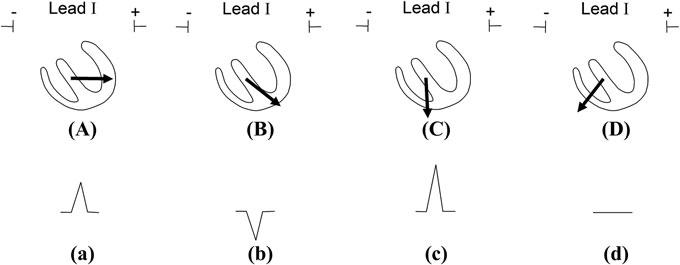
\includegraphics[width=0.8\textwidth]{1242.png}
  \caption{Ejemplos de dipolos cardíacos y derivación I de ECG (Basado en \cite{21}). Para los Problemas~12.30\text{--}12.32}
  \label{fig:12.42}
\end{figure}



\noindent \textbf{12.33} (a) Utilice la secuencia normal de evolución del dipolo cardíaco para bosquejar la evolución de la señal de ECG para las derivaciones I, II y III de ECG. \\
(b) Los potenciales de las tres derivaciones siempre deben sumar cero. Confirme que sus ECG lo hagan.

\noindent \textbf{12.34} Compare los ECG de la Fig.~12.37 ---tomados en dos momentos después de un ataque cardíaco--- entre sí y luego con los trazados normales de la Fig.~12.33.

\begin{thebibliography}{34}
\bibitem{1} B.K. Ahlborn, \textit{Zoological Physics: Quantitative Models, Body Design, Actions and Physical Limitations in Animals} (Springer, Berlín, 2004)
\bibitem{2} G.B. Benedek, F.M.H. Villars, \textit{Physics with Illustrative Examples from Medicine and Biology}, Tres volúmenes, 2.ª ed. (AIP/Springer, Nueva York, 2000)
\bibitem{3} B.H. Brown, R.H. Smallwood, D.C. Barber, P.V. Lawford, D.R. Hose, \textit{Medical Physics and Biomedical Engineering} (Institute of Physics, Filadelfia, 1999)
\bibitem{4} J.R. Cameron, J.G. Skofronick, R. Grant, \textit{Physics of the Body}, 2.ª ed. (Medical Physics, Madison, 1999)
\bibitem{5} R.M.J. Cotterill, \textit{Biophysics: An Introduction} (Wiley, Nueva York, 2002)
\bibitem{6} P. Davidovits, \textit{Physics in Biology and Medicine}, 2.ª ed. (Elsevier/Academic, San Diego, 2001)
\bibitem{7} T.A. Delcha, \textit{Physics in Medical Diagnosis} (Chapman \& Hall, Nueva York, 1997)
\bibitem{8} D. Dubin, \textit{Rapid Interpretation of EKG's}, 6.ª ed. (COVER, Tampa, 2000)
\bibitem{9} F.A. Duck, \textit{Physical Properties of Tissue: A Comprehensive Reference Book} (Academic, Londres, 1990)
\bibitem{10} G.L. Fain, \textit{Sensory Transduction} (Sinauer, Sunderland, 2003)
\bibitem{11} M.L. Foss, S.J. Keteyian, \textit{Fox's Physiological Basis for Exercise and Sport}, 6.ª ed. (McGraw-Hill, Boston, 1998)
\bibitem{12} R.A. Freitas Jr., \textit{Nanomedicine, Volume I: Basic Capabilities} (Landes Bioscience, Austin, 1999)
\bibitem{13} M. Gertsch, \textit{The ECG: A Two-Step Approach to Diagnosis} (Springer, Berlín, 2004)
\bibitem{14} N. Gimbel, C. Fox, \textit{Killing Me Softly (With His Song)}, escrita por Norman Gimbel y Charles Fox, publicada por Fox-Gimbel (BMI) y Rodali Music (BMI)
\bibitem{15} S. Grimnes, \O{}.G. Martinsen, \textit{Bioimpedance and Bioelectricity Basics} (Academic, San Diego, 2000)
\bibitem{16} A.C. Guyton, J.E. Hall, \textit{Human Physiology and Mechanisms of Disease}, 6.ª ed. (Saunders, Filadelfia, 1997)
\bibitem{17} R.K. Hobbie, \textit{Intermediate Physics for Medicine and Biology}, 3.ª ed. (AIP, Nueva York, 1997)
\bibitem{18} R.K. Hobbie, B.J. Roth, \textit{Intermediate Physics for Medicine and Biology}, 4.ª ed. (Springer, Berlín, 2007)
\bibitem{19} F.C. Hoppensteadt, C.S. Peskin, \textit{Modeling and Simulation in Medicine and the Life Sciences}, 2.ª ed. (Springer, Nueva York, 2002) (La primera edición de 1992 se llamó \textit{Mathematics in Medicine and the Life Sciences})
\bibitem{20} A.J. Hudspeth, D.P. Corey, Sensitivity, polarity, and conductance change in the response of vertebrate hair cells to controlled mechanical stimuli. \textit{Proc. Natl. Acad. Sci. USA} \textbf{74}, 2407--2411 (1977)
\bibitem{21} L.S. Lilly, The electrocardiogram, en \textit{Pathophysiology of Heart Disease: A Collaborative Project of Medical Students and Faculty}, 3.ª ed., ed. por L.S. Lilly (Lippincott Williams \& Wilkins, Filadelfia, 2003), Cap. 4, pp. 75--110
\bibitem{22} R. Malhotra, E.R. Edelman, Basic cardiac structure and function, en \textit{Pathophysiology of Heart Disease: A Collaborative Project of Medical Students and Faculty}, 3.ª ed., ed. por L.S. Lilly (Lippincott Williams \& Wilkins, Filadelfia, 2003), Cap. 1, pp. 1--27
\bibitem{23} J. Malmivuo, R. Plonsey, \textit{Bioelectromagnetism} (Oxford University Press, Nueva York, 1995)
\bibitem{24} H.J. Metcalf, \textit{Topics in Classical Biophysics} (Prentice-Hall, Englewood Cliffs, 1980)
\bibitem{25} K.L. Moore, A.M.R. Agur, \textit{Essential Clinical Anatomy}, 3.ª ed. (Lippincott Williams \& Wilkins, Filadelfia, 2007)
\bibitem{26} W. Rall, Cable theory for dendritic neurons, en \textit{Methods in Neuronal Modeling: From Synapses to Networks}, ed. por C. Koch, et al., I. Segev (MIT, Cambridge, 1989), Cap. 2, pp. 9--62
\bibitem{27} R.M. Ross, A.S. Jackson, \textit{Exercise Concepts, Calculations, and Computer Applications} (Benchmark, Carmel, 1990)
\bibitem{28} A.M. Scher, The electrocardiogram, en \textit{Textbook of Physiology}, 21.ª ed., ed. por H.D. Patton, A.F. Fuchs, B. Hille, A.M. Scher, R. Steiner (Saunders, Filadelfia, 1989), Cap. 38, pp. 796--819
\bibitem{29} T.H. Schiebler, \textit{Anatomie}, 9.ª ed. (Springer, Berlín, 2005)
\bibitem{30} R.F. Schmidt, F. Lang, G. Thews, \textit{Physiologie des Menschen}, 29.ª ed. (Springer, Berlín, 2005)
\bibitem{31} A. Stalheim-Smith, G.K. Fitch, \textit{Understanding Human Anatomy and Physiology} (West, St. Paul, 1993)
\bibitem{32} Thomas Jefferson National Accelerator Facility (U.S.), \textit{Jefferson Lab Environment, Safety, Health, and Quality Manual}. \url{http://www.jlab.org/ehs/manual/EHSbook-429.html}
\bibitem{33} J.A. Tuszynski, J.M. Dixon, \textit{Biomedical Applications of Introductory Physics} (Wiley, Nueva York, 2002)
\bibitem{34} J.B. West (ed.), \textit{Best and Taylor's Physiological Basis of Medical Practice}, 12.ª ed. (Williams \& Wilkins, Baltimore, 1991)
\end{thebibliography}

% Control de Calidad: 43 párrafos origen -> 43 párrafos salida. Mapeo 1:1 verificado. Sin omisiones.

\end{document}
